\documentclass[aspectratio=169]{beamer} 

\usepackage{hayesmacros}
\usepackage{appendixnumberbeamer}
\usepackage{subcaption}

\usetheme[numbering=fraction, block=fill]{metropolis}
\setsansfont{Fira Sans}  % be sure to compile with XeLaTeX

\usepackage{natbib}
\usepackage{ulem}
\usepackage{fontawesome5}

\newtheorem{proposition}{Proposition}
\newtheorem{assumption}{Assumption}

\theoremstyle{remark}
\newtheorem*{remark}{Remark}

\setbeamercolor{background canvas}{bg=white}
\setbeamercolor{normal text}{fg=black}
\setbeamercolor{frametitle}{bg=black, fg=white}

\hypersetup{colorlinks,citecolor=cyan, urlcolor=cyan, linkcolor=black}

\title{Estimating network-mediated causal effects via spectral embeddings}

\date{2024-06-17}
\author{Alex Hayes}
\institute{University of Wisconsin-Madison}


\begin{document}

\maketitle

{
    \usebackgroundtemplate{
\includegraphics[width=\paperwidth, height=\paperheight]{./figures/hm-app.png}}
    \begin{frame}
    \end{frame}
}

\begin{frame}{Experiments (n = 662) show that smartphone-guided meditation reduces anxiety}
    \begin{figure}
        \centering
        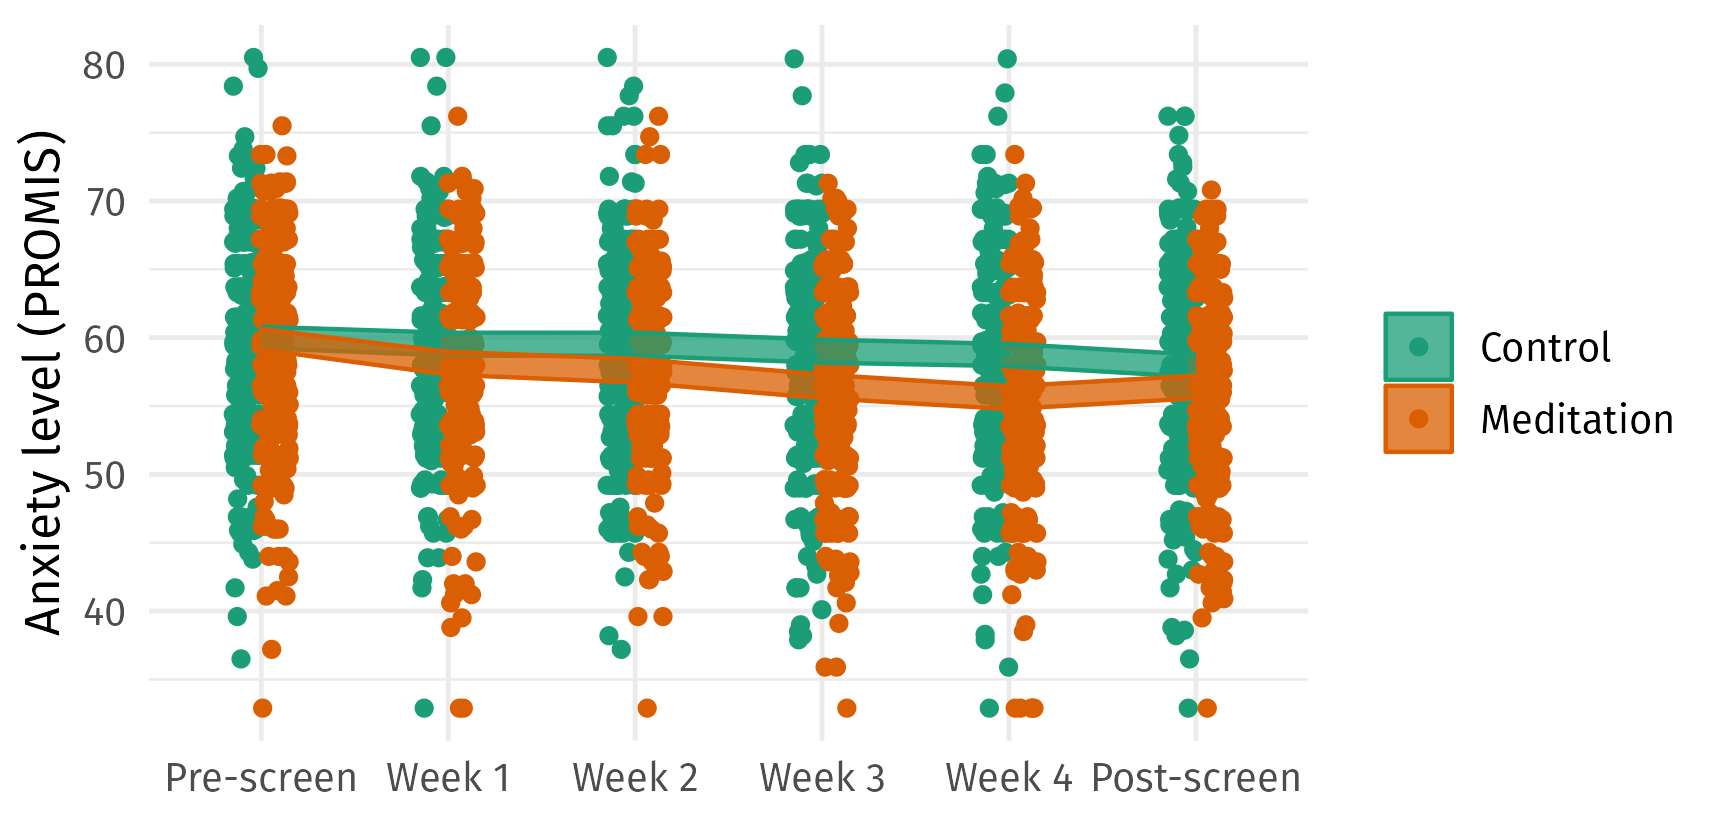
\includegraphics{./figures/ate.png}
    \end{figure}
\end{frame}

\begin{frame}{We study the causal effect of four weeks of meditation}

    \begin{columns}
        \column{0.6 \textwidth}

        Counterfactual outcomes

        \begin{table}[]
            \begin{tabular}{lcl}
                anxiety, no meditation & $Y_i(0)$ & $\in \R$ \\
                anxiety, meditation    & $Y_i(1)$ & $\in \R$
            \end{tabular}
        \end{table}

        Observed data

        \begin{table}[]
            \begin{tabular}{lcrl}
                Treatment & meditation & $T_i$ & $\in \set{0, 1} $ \\
                Outcome   & anxiety    & $Y_i$ & $\in \R$
            \end{tabular}
        \end{table}
        \begin{align*}
            \ate    & = \E{Y_i (1) - Y_i (0)}                       \\
                    & = \E{Y_i \mid T_i = 1} - \E{Y_i \mid T_i = 0} \\
            \atehat & = -2.7 \pm 1.3
        \end{align*}

        \column{0.4 \textwidth}
        \centering
        \begin{figure}[ht]
            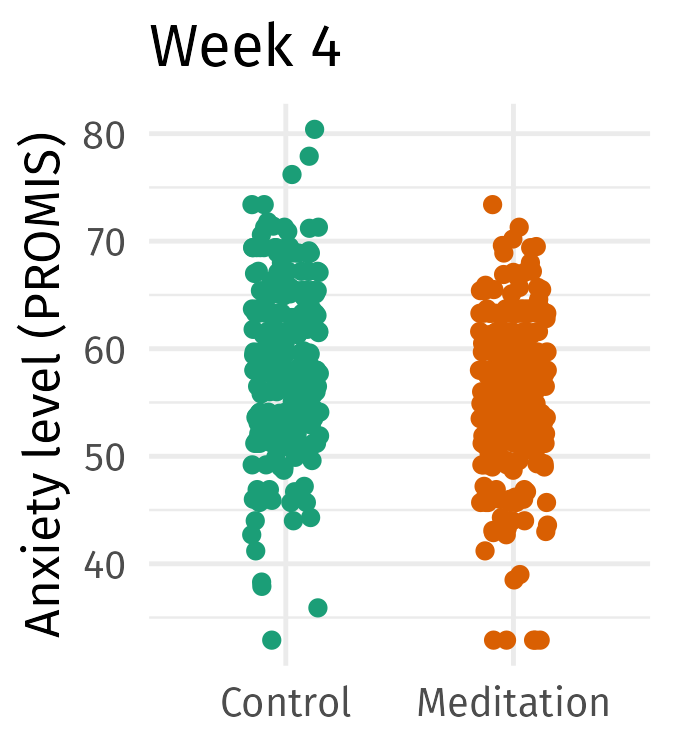
\includegraphics{figures/week4_scatter.png}
            \centering
        \end{figure}
    \end{columns}
\end{frame}

\begin{frame}{Psychologists want to know \underline{why} the Healthy Minds Program reduces distress}

    The meditation program is designed to alter latent cognitive factors

    \begin{enumerate}
        \item Awareness (mindful action)
        \item Connection (social connection, reducing loneliness)
        \item Insight (cognitive defusion)
        \item Purpose (presence of meaning)
    \end{enumerate}

    The hope: improving these latent cognitive factors reduces anxiety
\end{frame}

\begin{frame}{Multi-stage effects can be formalized as causal mediation}
    \begin{columns}
        \column{0.67 \textwidth}
        Decompose effect of $T_i$ on $Y_i$:

        \vspace{4mm}

        \begin{enumerate}
            \item Effect operating along $T_i \to Y_i$ path (direct)
                  \begin{itemize}
                      \item i.e., guided breathing reduces anxiety
                  \end{itemize}
                  \vspace{2mm}
            \item Effect operating along $T_i \to \X_{i \cdot} \to Y_i$ path (indirect)

                  \begin{itemize}
                      \item i.e., meditation program decreases loneliness, which in turn decreases anxiety
                  \end{itemize}
        \end{enumerate}

        \begin{equation*}
            \ate = \nde + \nie
        \end{equation*}
        \column{0.32 \textwidth}
        \centering
        \begin{figure}[ht]
            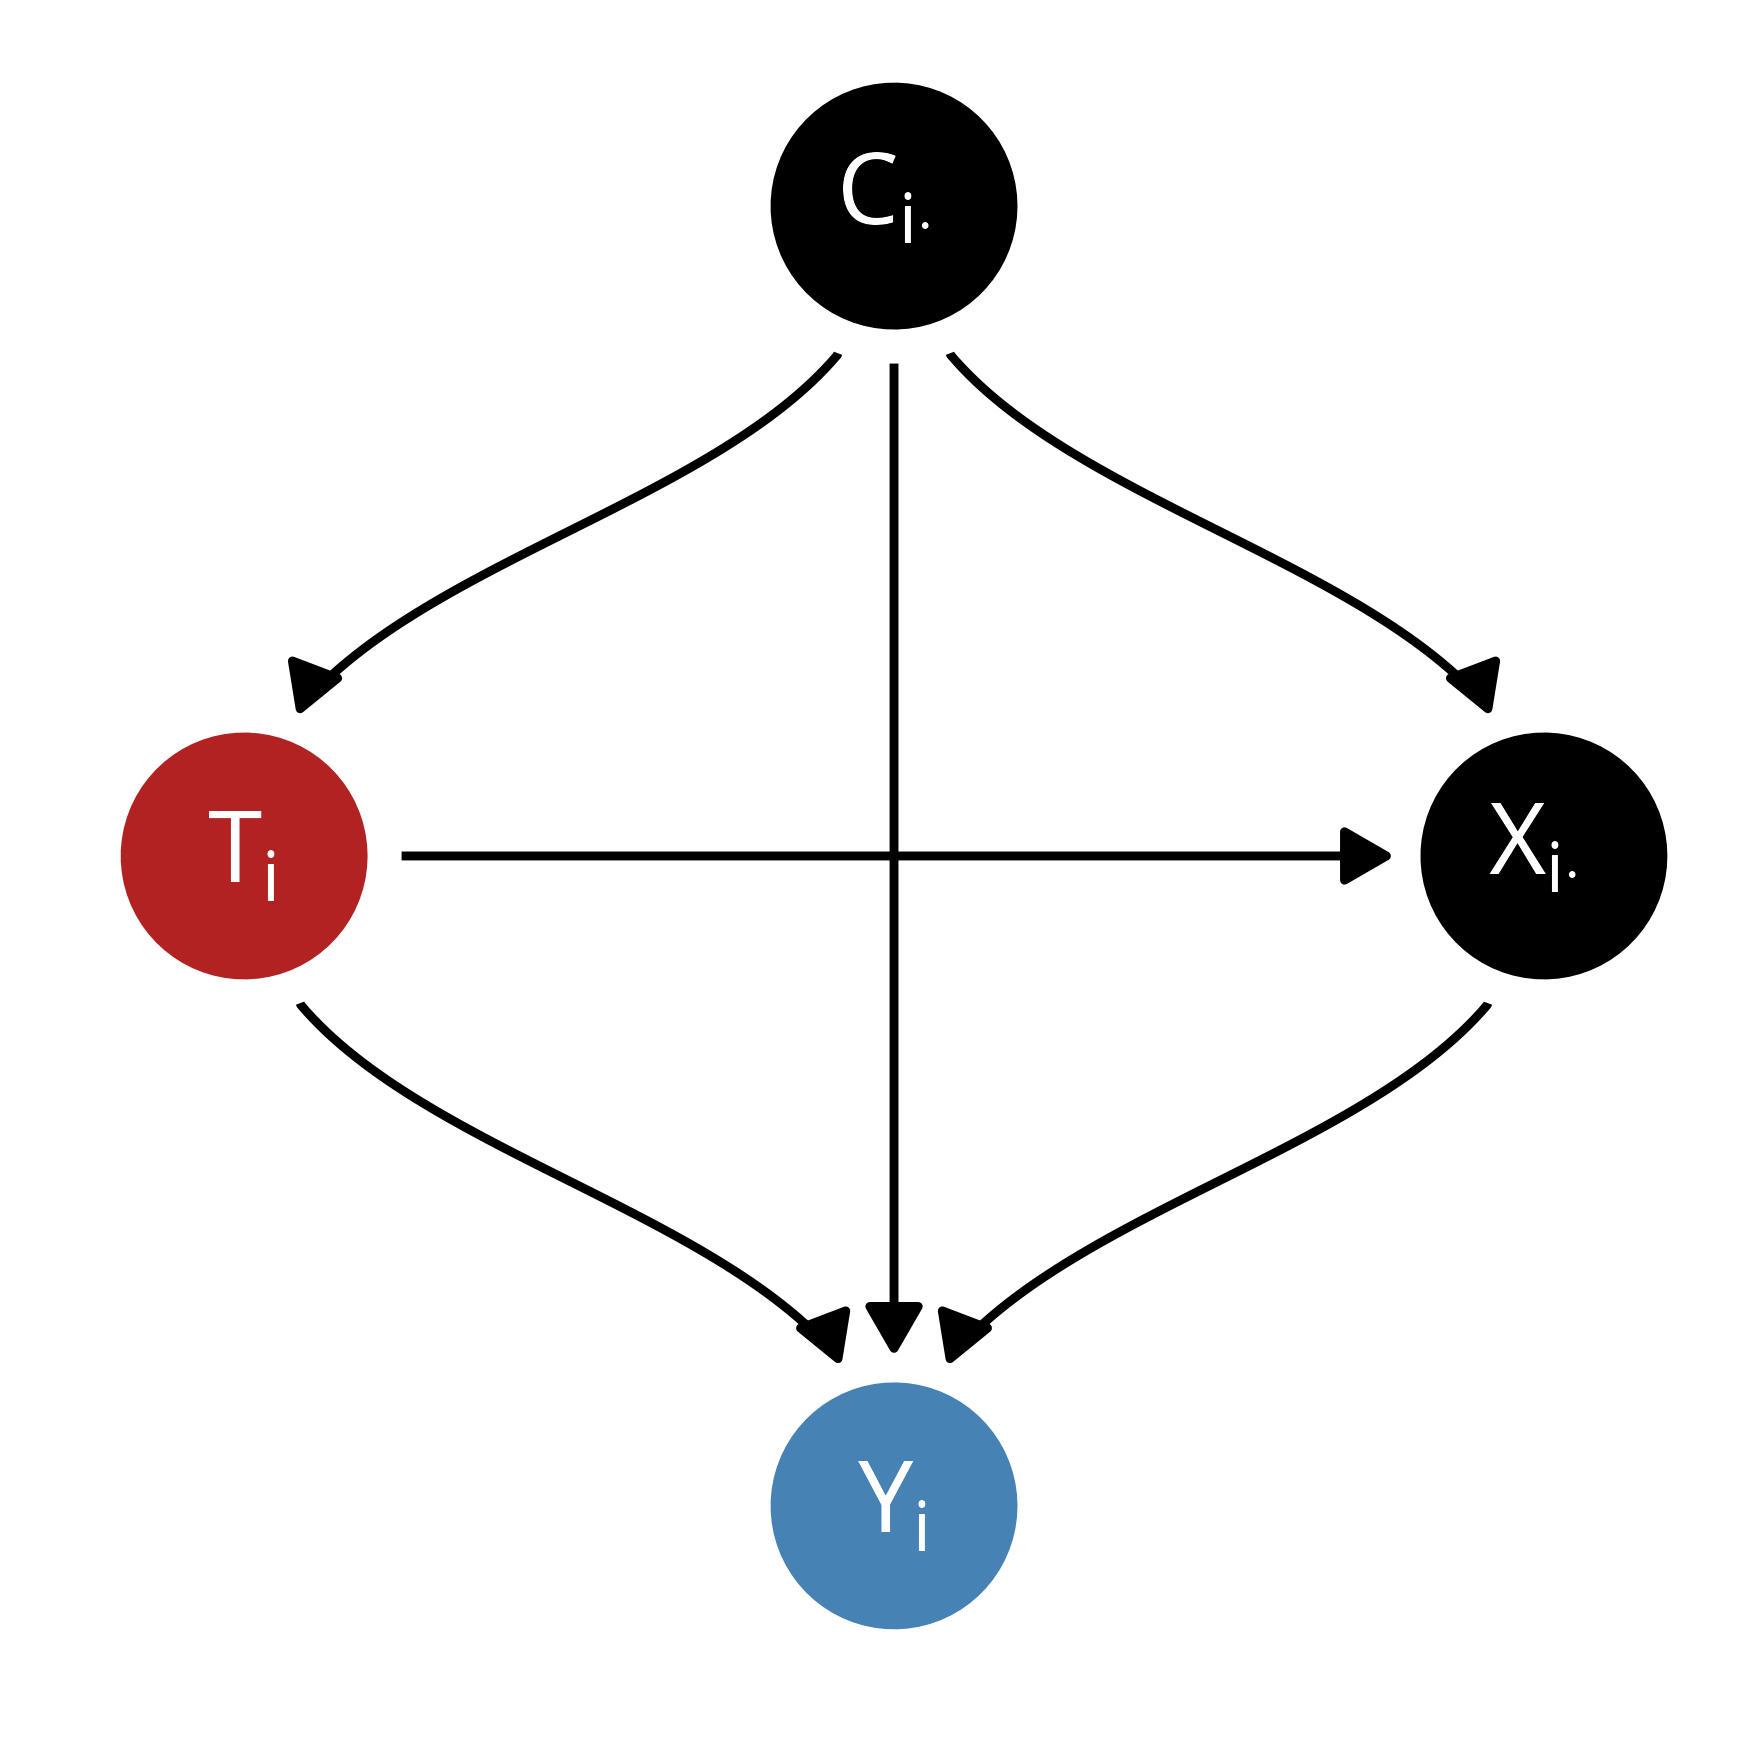
\includegraphics[width=\textwidth]{figures/dags/mediating.png}
        \end{figure}
    \end{columns}
\end{frame}

\begin{frame}{Natural direct and indirect effects are defined counterfactually}
    \begin{columns}
        \column{0.67 \textwidth}
        \begin{table}[]
            \begin{tabular}{lcrl}
                Treatment   & meditation      & $T_i$          & $\in \set{0, 1} $     \\
                Outcome     & anxiety         & $Y_i$          & $\in \R$              \\
                Mediators   & cognitive state & $\X_{i \cdot}$ & $\in \R^{1 \times d}$ \\
                Confounders & age \& sex      & $\C_{i \cdot}$ & $\in \R^{1 \times p}$
            \end{tabular}
        \end{table}
        \begin{align*}
            \nde & = \E{Y_i (t, \X_{i \cdot}(t^*)) - Y_i (t^*, \X_{i \cdot} (t^*))} \\
            \nie & = \E{Y_i (t, \X_{i \cdot}(t)) - Y_i (t, \X_{i \cdot} (t^*))}
        \end{align*}

        If we knew cognitive state, we could use standard tools. But cognitive state is latent!
        \column{0.33 \textwidth}
        \centering
        \begin{figure}[ht]
            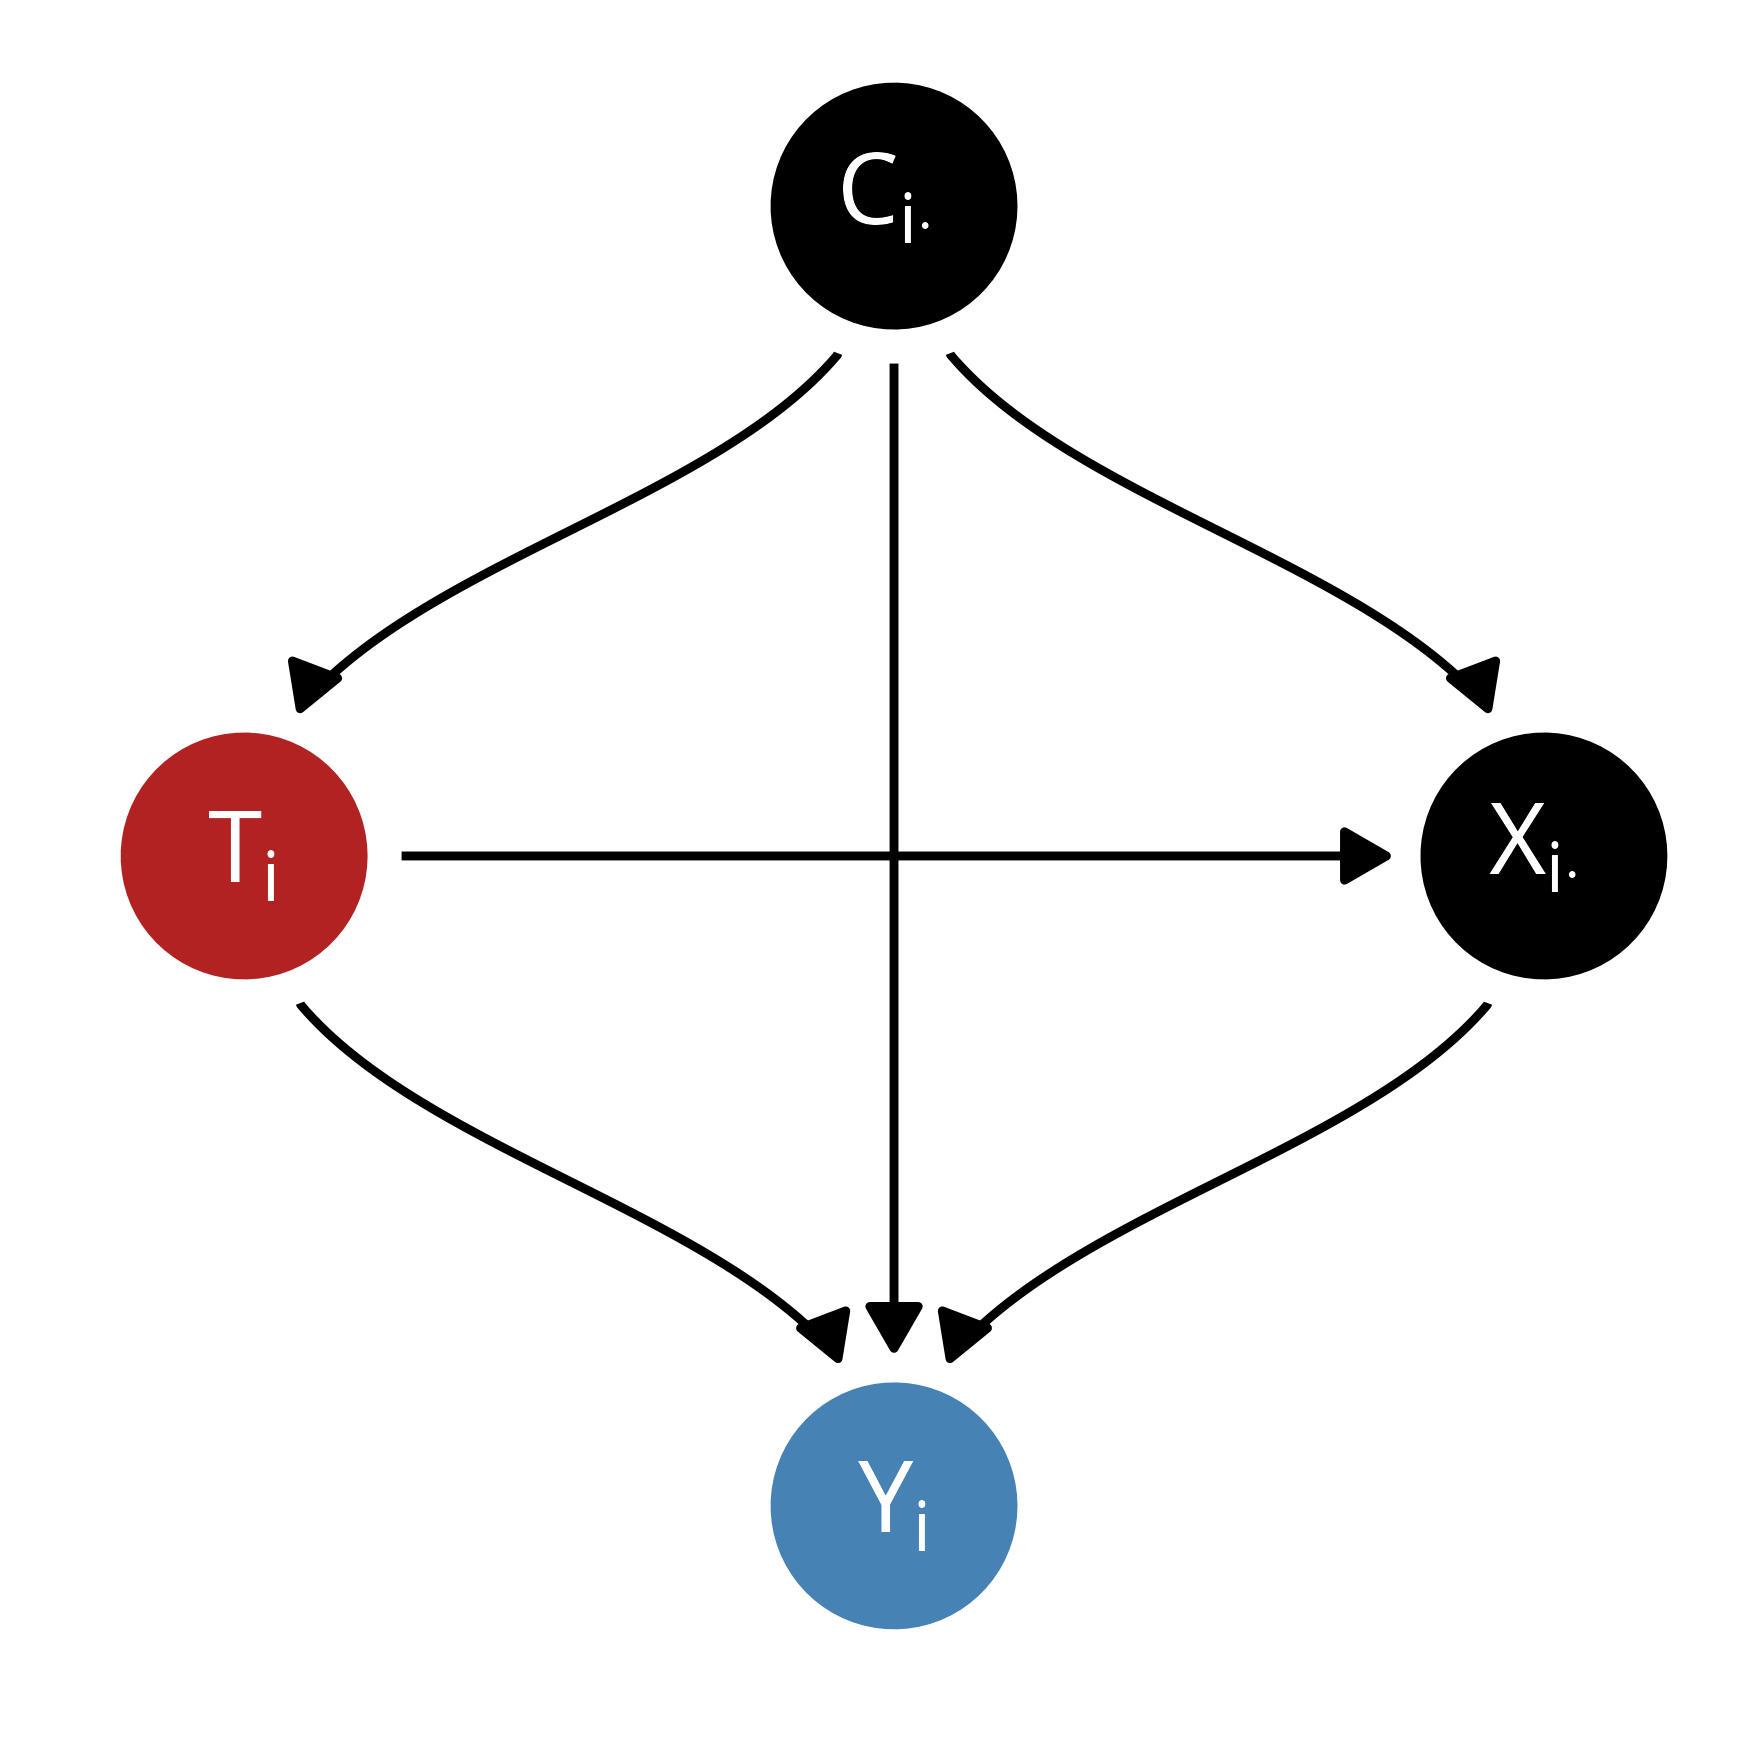
\includegraphics[width=\textwidth]{figures/dags/mediating.png}
            \centering
        \end{figure}
    \end{columns}
\end{frame}

\begin{frame}{Psychologists measure latent cognitive state using surveys}

    For example, the NIH Toolbox loneliness survey

    \begin{enumerate}
        \item I feel alone and apart from others
        \item I feel left out
        \item I feel that I am no longer close to anyone
        \item I feel alone
        \item I feel lonely
    \end{enumerate}

    \begin{table}[]
        \begin{tabular}{ccccc}
            Never                      & Rarely                     & Sometimes                  & Usually                    & Always                     \\
            1 \faIcon[regular]{circle} & 2 \faIcon[regular]{circle} & 3 \faIcon[regular]{circle} & 4 \faIcon[regular]{circle} & 5 \faIcon[regular]{circle}
        \end{tabular}
    \end{table}
\end{frame}

\begin{frame}{The experimenters ran weekly surveys of the study participants}

    \begin{itemize}
        \item NIH Toolbox Loneliness (5 questions)
        \item Five Facet Mindfulness Questionnaire Acting with Awareness subscale (8 questions)
        \item Drexel Defusion Scale (10 questions)
        \item Meaning in Life Questionnaire (10 questions)
    \end{itemize}
\end{frame}

\begin{frame}{Another survey: the Meaning in Life Questionnaire}

    \begin{enumerate}
        \item I understand my life's meaning.
        \item I am looking for something that makes my life feel meaningful.
        \item I am always looking to find my life's purpose.
        \item My life has a clear sense of purpose.
        \item I have a good sense of what makes my life meaningful.
        \item I have discovered a satisfying life purpose.
        \item I am always searching for something that makes my life feel significant.
        \item I am seeking a purpose or mission for my life
        \item My life has no clear purpose.
        \item I am searching for meaning in my life.
    \end{enumerate}

    \footnotesize
    \resizebox{\linewidth}{!}{
        \begin{tabular}{ccccccc}
            Absolutely untrue          & Mostly untrue              & Somewhat untrue            & Can't say true or false    & Somewhat true              & Mostly true                & Absolutely true            \\
            1 \faIcon[regular]{circle} & 2 \faIcon[regular]{circle} & 3 \faIcon[regular]{circle} & 4 \faIcon[regular]{circle} & 5 \faIcon[regular]{circle} & 6 \faIcon[regular]{circle} & 7 \faIcon[regular]{circle}
        \end{tabular}
    }
\end{frame}

\begin{frame}{The survey responses form a bipartite network}
    \centering
    \begin{figure}
        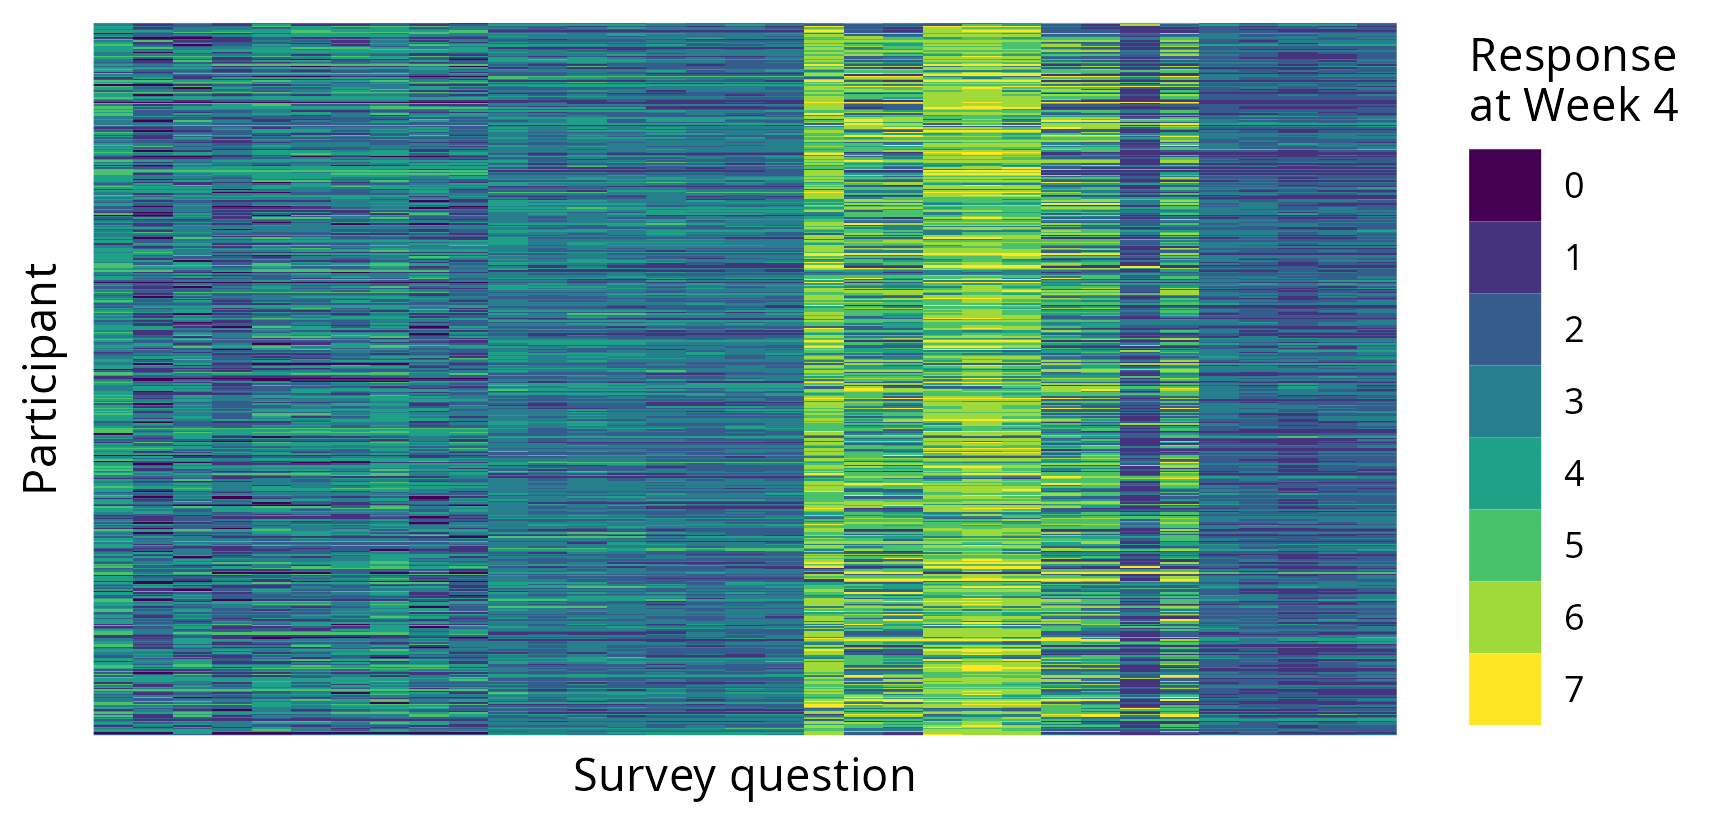
\includegraphics{figures/week4-responses.png}
    \end{figure}
\end{frame}

\begin{frame}{We model survey responses using a factor model}

    Suppose $A \in \R^{n \times m}$ is the matrix of survey responses. Then

    \begin{equation*}
        \E[X, Z]{A} = X Z^T
    \end{equation*}

    \begin{table}[]
        \begin{tabular}{lcl}
            Participant embeddings & $X$ & $\in \R^{n \times d}$ \\
            Question embeddings    & $Z$ & $\in \R^{m \times d}$
        \end{tabular}
    \end{table}

\end{frame}

\begin{frame}{We estimate latent cognitive state by embedding the network}

    \begin{definition}[ASE]

        Given a network $A$, the $d$-dimensional \emph{adjacency spectral embeddings} of $A$ is
        \begin{align*}
            \Xhat = \Uhat \Shat^{1/2} ~\text{ and } \widehat{Z} = \Vhat \Shat^{1/2}
        \end{align*}
        \noindent where $\Uhat \Shat \Vhat^T$ is the rank-$d$ truncated singular value decomposition of $A$.
    \end{definition}

    \begin{lemma}
        Under a suitable low-rank model, there are $d \times d$ orthogonal matrices $Q_1, Q_2$ such that
        % TODO: is it the same Q for both the left and right co-factors
        \begin{equation*}
            \max_{i \in [n]} \, \norm*{\Xhat_{i \cdot} - \X_{i \cdot} Q_1} = \op{1}
            ~\text{ and }~
            \max_{i \in [n]} \, \norm*{\Vhat_{i \cdot} - V_{i \cdot} Q_2} = \op{1}.
        \end{equation*}
    \end{lemma}
\end{frame}


\begin{frame}{We must estimate the number of latent factors $d$}
    \centering
    \begin{figure}
        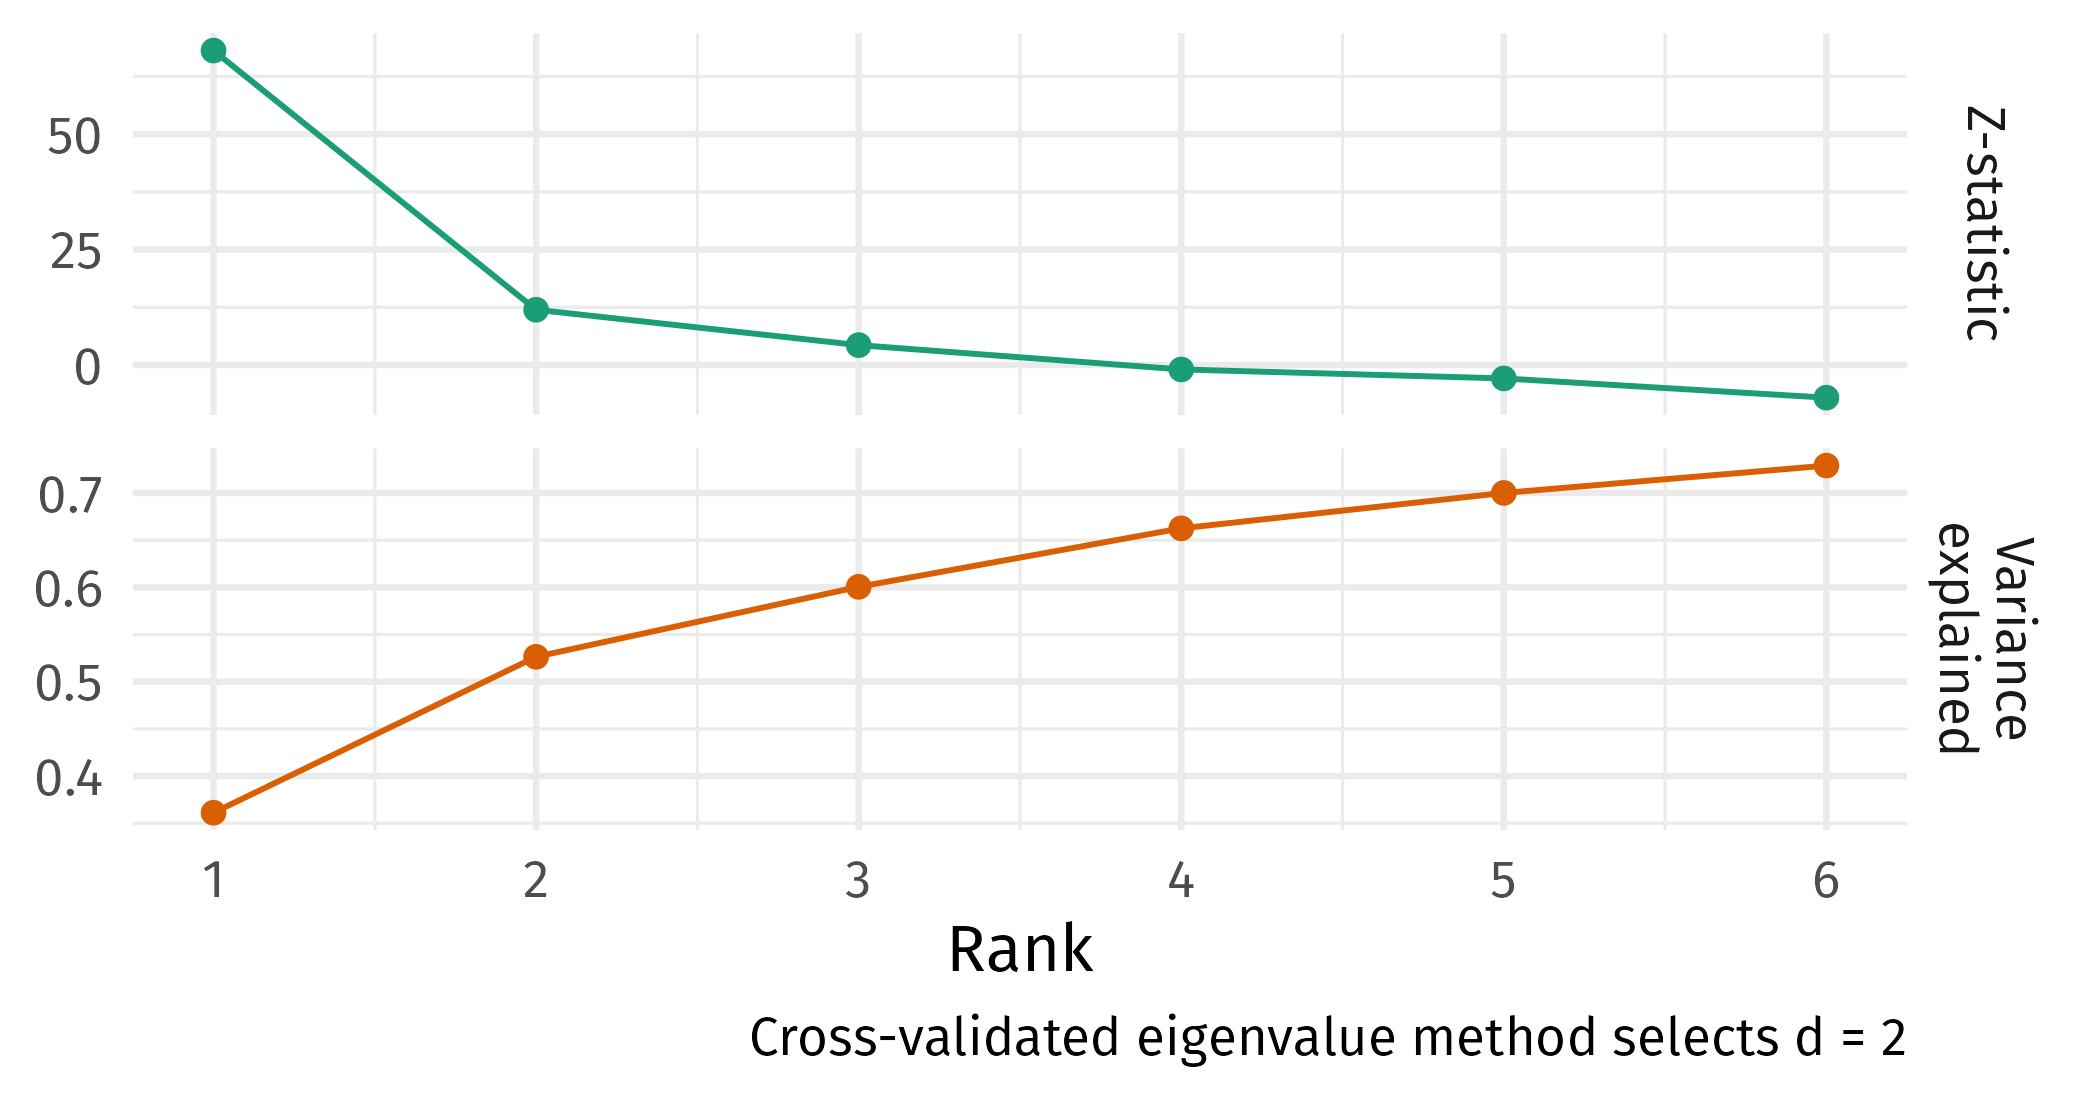
\includegraphics{figures/rank-determination.png}
    \end{figure}
\end{frame}

\begin{frame}{Participants embed into an inocuous latent space}
    \centering
    \begin{figure}
        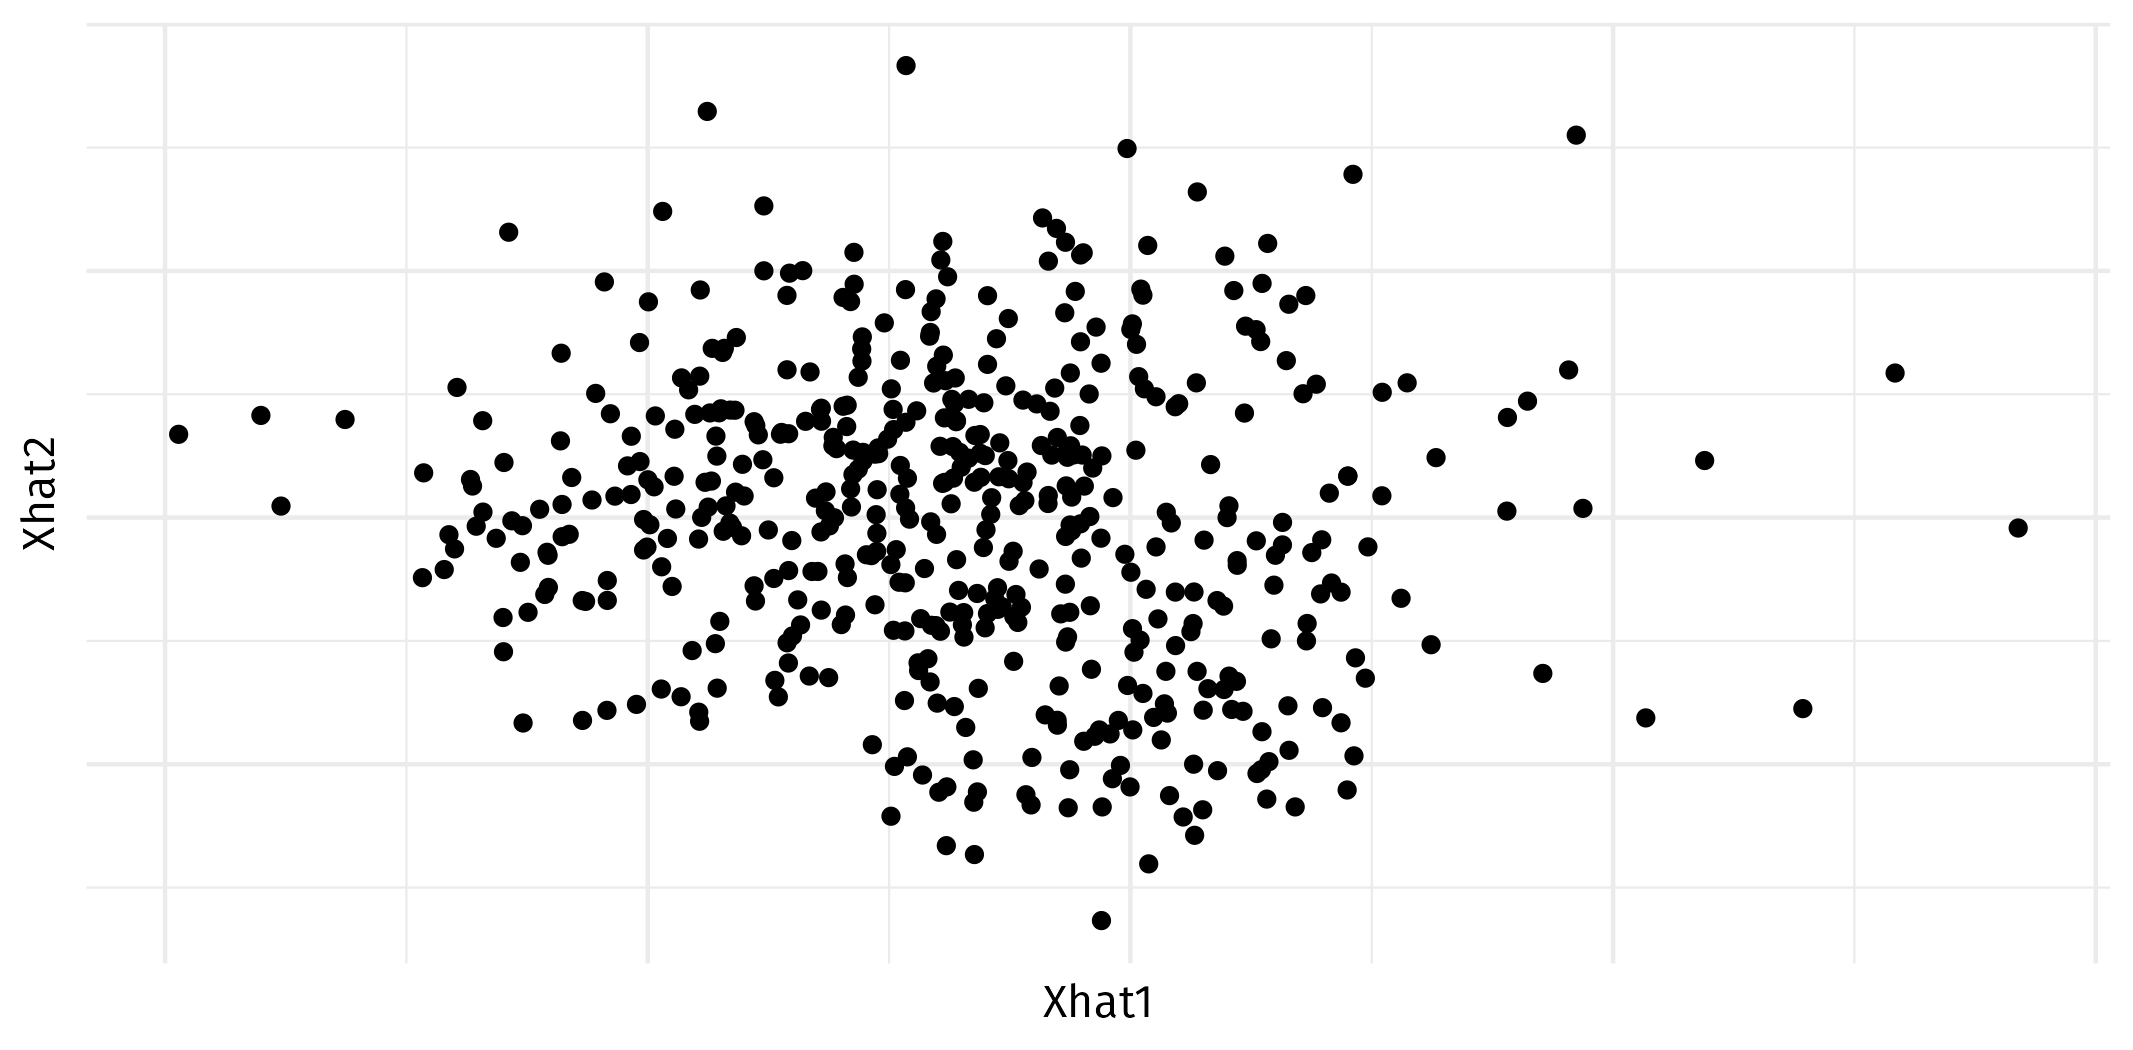
\includegraphics[width=\textwidth]{figures/xhat.png}
    \end{figure}
\end{frame}

\begin{frame}{The survey questions are largely redundant}
    \begin{figure}
        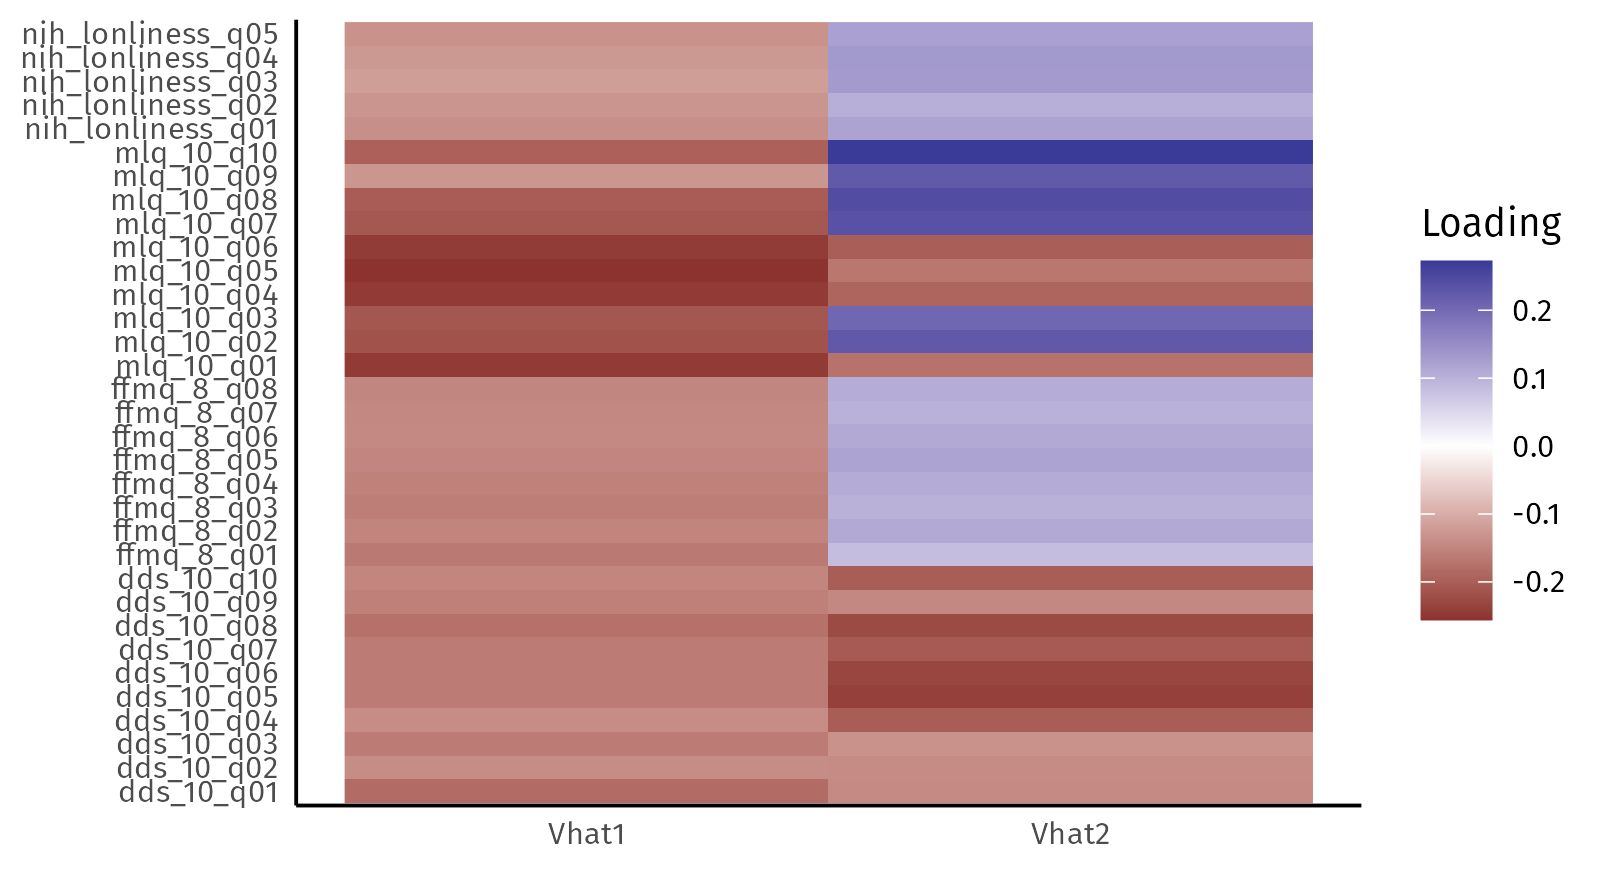
\includegraphics{figures/vhat.png}
    \end{figure}
\end{frame}

\begin{frame}{Recap so far}

    \begin{itemize}
        \item Psychologists hoped to find four latent factors corresponding to loneliness, meaning in life, etc, etc
        \item We only found two "do you feel good", and "do you feel bad"
        \item People basically answer all the questions exactly the same
        \item Still curious how much the latent well-being factors account for decrease in anxiety
    \end{itemize}

\end{frame}

\begin{frame}{We use survey responses to estimate latent participant embeedings}
    \centering
    \begin{figure}
        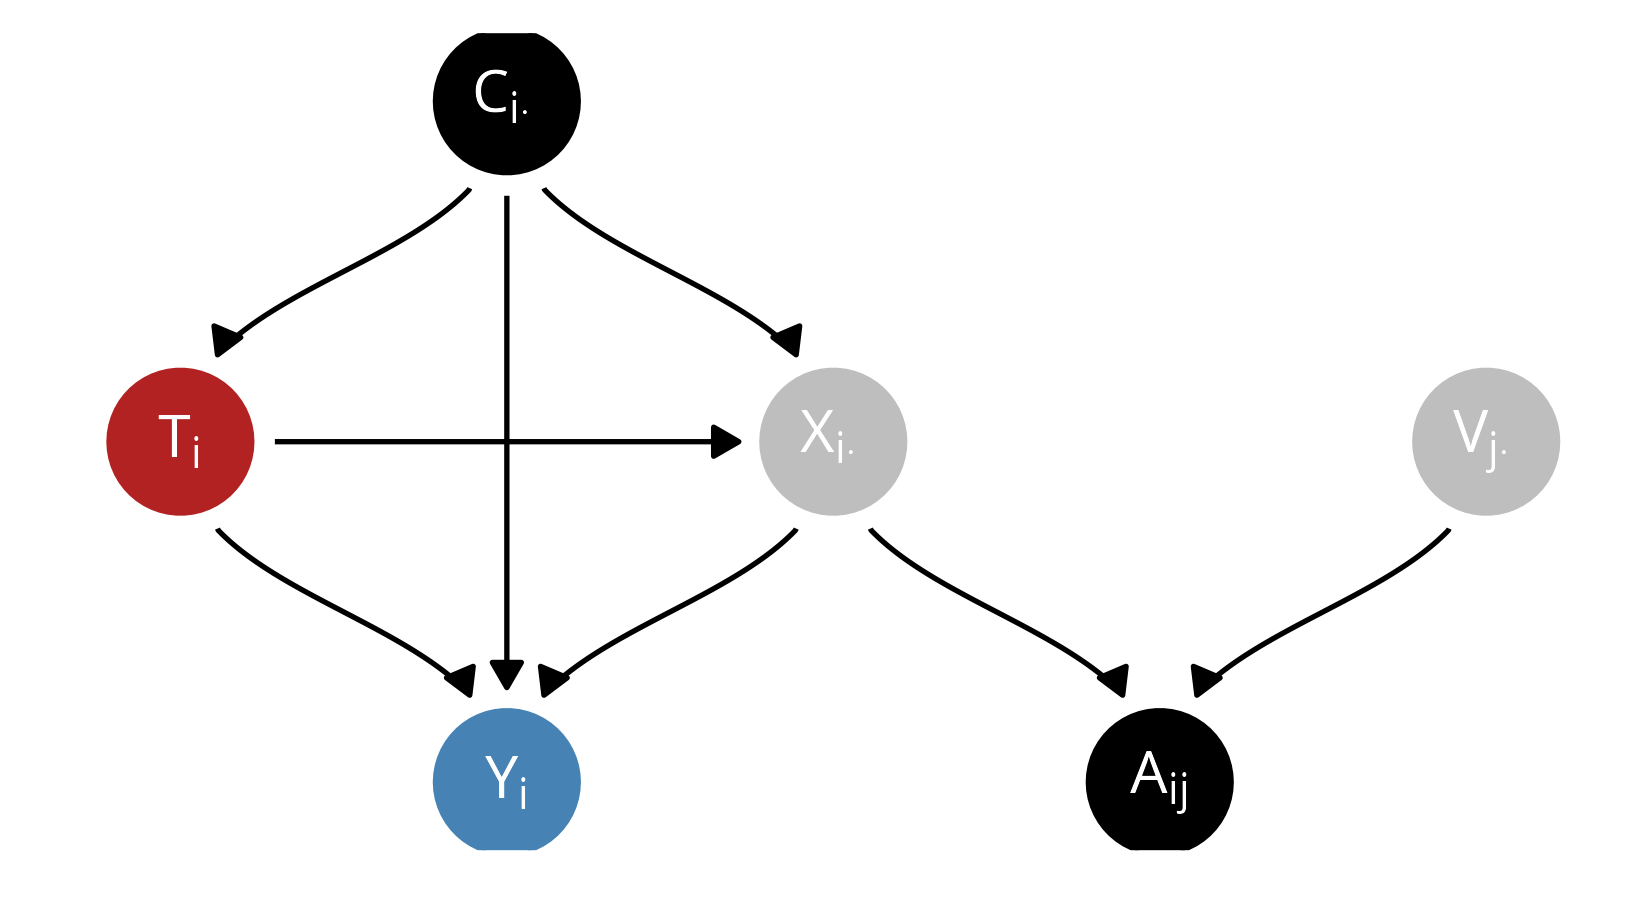
\includegraphics[width=\textwidth]{figures/dags/bipartite-mediation.png}
    \end{figure}
\end{frame}


\begin{frame}{The identifying assumptions can be expressed counterfactually}

    The random variables $(Y_i, Y_i(t, x), \X_{i \cdot}, \X_{i \cdot}(t), C_{i \cdot}, T_i)$ are independent over $i \in [n]$ and obey the following three properties.
    \begin{enumerate}
        \item Consistency: \vspace{-3mm}
              \begin{equation*} \begin{aligned}
                       & \text{if $T_i = t$, then $\X_{i \cdot}(t) = \X_{i \cdot}$ with probability 1, and}    \\
                       & \text{if $T_i = t$ and $\X_{i \cdot} = x$, then $Y_i(t, x) = Y_i$ with probability 1}
                      \vspace{-2mm}
                  \end{aligned} \end{equation*}
        \item Sequential ignorability:
              \begin{equation*}
                  \set{Y_i(t^*, x), \X_{i \cdot}(t)} \indep T_i \cond \C_{i \cdot}
                  ~~~\text{ and }~~~
                  \set{Y_i(t^*, x)} \indep \X_{i \cdot}  \cond T_i = t, \C_{i \cdot}
              \end{equation*}
        \item Positivity:
              \begin{equation*}
                  \begin{aligned}
                      \P[T_i, \C_{i \cdot}]{x} & > 0 \text{ for each }  x \in \supp(\X_{i \cdot}) \\
                      \P[\C_{i \cdot}]{t}      & > 0 \text{ for each }  t \in \supp(T_i)
                  \end{aligned}
              \end{equation*}
    \end{enumerate}

\end{frame}

\begin{frame}{Under semi-parametric assumptions, causal effects are regression coefficients}

    If the non-parametric identification conditions hold and also
    \begin{equation*}
        \begin{aligned}
            \underbrace{\E[T_i, \C_{i \cdot}, \X_{i \cdot}]{Y_i}}_{\R}
             & = \underbrace{\betazero}_{\R}
            + \underbrace{T_i}_{\{0, 1\}} \underbrace{\betat}_{\R}
            + \underbrace{\C_{i \cdot}}_{\R^{1 \times p}} \underbrace{\betac}_{\R^{p}}
            + \underbrace{\X_{i \cdot}}_{\R^{1 \times d}} \underbrace{\betax}_{\R^d}, \\
            \underbrace{\E[T_i, \C_{i \cdot}]{\X_{i \cdot}}}_{\R^{1 \times d}}
             & = \underbrace{\thetazero}_{\R^{1 \times d}}
            + \underbrace{T_i}_{\{0, 1\}} \underbrace{\thetat}_{\R^{1 \times d}}
            + \underbrace{\C_{i \cdot}}_{\R^{1 \times p}} \underbrace{\Thetac}_{\R^{p \times d}}
        \end{aligned}
    \end{equation*}
    Then
    \begin{align*}
        \ndef & = \paren*{t - t^*} \, \betat            \\
        \nief & = \paren*{t - t^*} \, \thetat \, \betax
    \end{align*}

\end{frame}

\begin{frame}{We using estimated $\Xhat$ in place of unobserved $\X$ in regression estimators}
    Let $\Dhat = \begin{bmatrix} 1 & T & \C  & \Xhat \end{bmatrix} \in \R^{n \times (2 + p + d)}$ and $\Wfull = \begin{bmatrix} 1 & T & \C \end{bmatrix} \in \R^{n \times (p + 2)}$.
    \begin{equation*}
        \begin{bmatrix}
            \betazerohat \\
            \betathat    \\
            \betachat    \\
            \betaxhat
        \end{bmatrix}
        = \paren*{\Dhat^T \Dhat}^{-1} \Dhat^T Y
        \quad \text{and} \quad
        \Thetahat
        = \paren*{\Wfull^T \Wfull}^{-1} \Wfull^T \Xhat.
    \end{equation*}

    \begin{align*}
        \ndehat & = \paren*{t - t^*} \, \betathat               \\
        \niehat & = \paren*{t - t^*} \, \thetathat \, \betaxhat
    \end{align*}
\end{frame}

\begin{frame}{Regression coefficients are asymptotically normal}

    \begin{theorem}

        \vspace{2mm}

        Under a suitably well-behaved network model and some moment conditions on regression errors, there is an unknown orthogonal matrix $Q$ such that
        \begin{equation*}
            \begin{aligned}
                \sqrt{ n } \,
                 & \Sigmahatbeta^{-1/2}
                \begin{pmatrix}
                    \betawhat - \betaw \\
                    Q \, \betaxhat - \betax
                \end{pmatrix}
                \to
                \Normal{0}{I_d}, and     \\
                \sqrt{ n } \,
                 & \Sigmahattheta^{-1/2}
                \begin{pmatrix}
                    \vecc \paren*{\Thetahat \, Q^T} - \Thetavec
                \end{pmatrix}
                \to
                \Normal{0}{I_{p d}}.
            \end{aligned}
        \end{equation*}
        \noindent where $\Sigmahattheta^{-1/2}$ and $\Sigmahatbeta^{-1/2}$ are the typical heteroscedasticity robust covariance estimators, with $\Xhat$ plugged in for $\X$.
    \end{theorem}
\end{frame}

\begin{frame}{Causal estimators are asymptotically normal}

    \begin{theorem}
        \vspace{2mm}

        Under the same statistical assumptions as before, plus mediating homophily,
        \begin{align*}
            \sqrt{n \, \sigmahatnde} \paren*{\ndehat - \nde}
             & \to
            \Normal{0}{1}, \text { and } \\
            \sqrt{n \, \sigmahatnie} \paren*{\niehat - \nie}
             & \to
            \Normal{0}{1}.
        \end{align*}
        \noindent where $\sigmahatnde$ and $\sigmahatnie$ are variance estimators derived via the delta method and the previous theorem.

    \end{theorem}

\end{frame}

\begin{frame}{Latent factors increase anxiety, meditation decreases anxiety}
    \centering
    \begin{figure}
        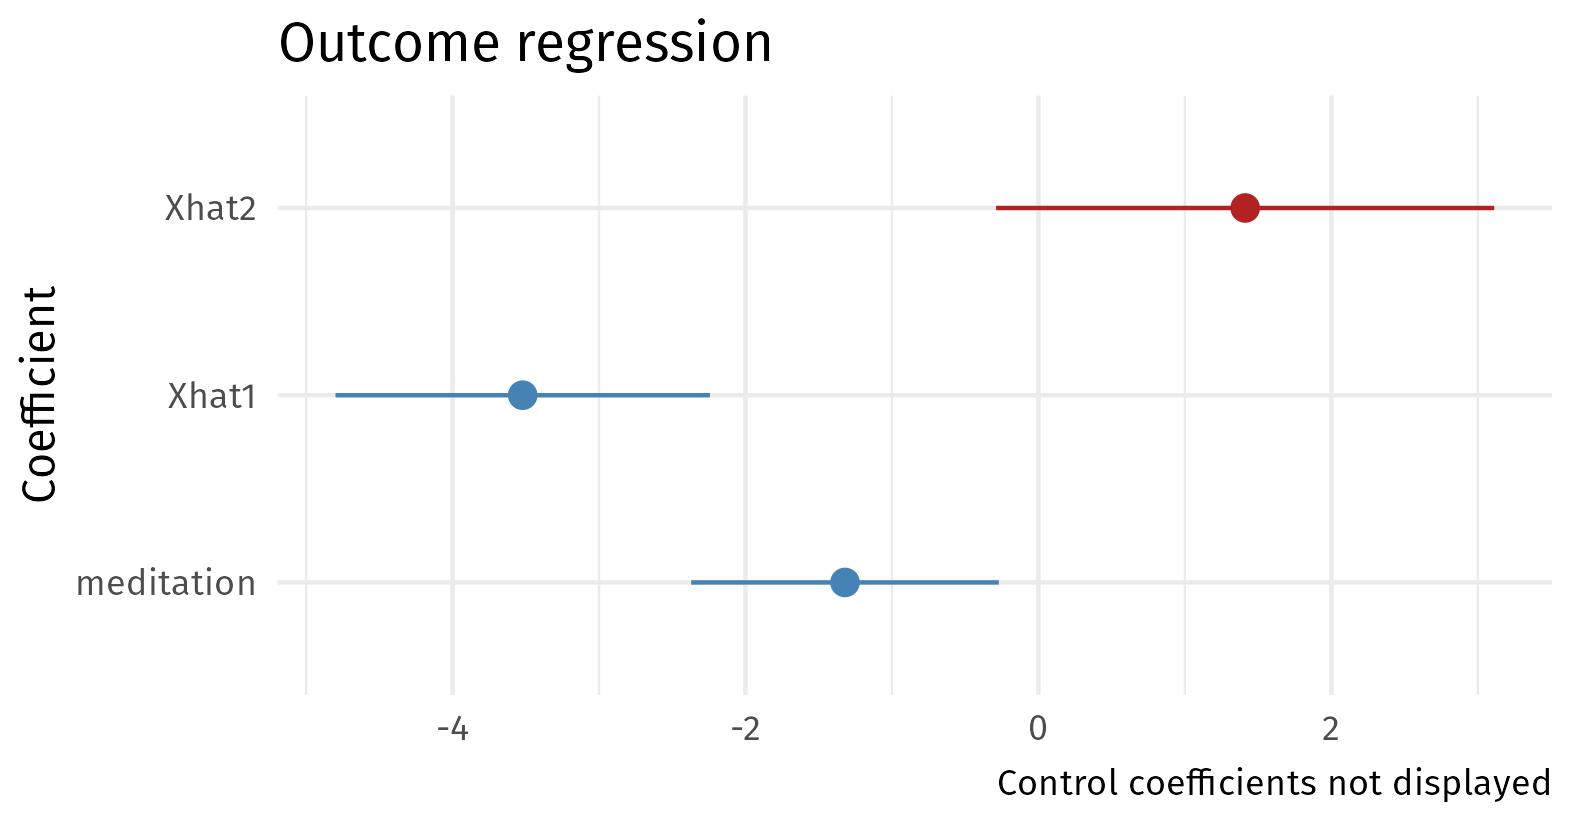
\includegraphics[width=\textwidth]{figures/outcome-coefficients.png}
    \end{figure}
\end{frame}

\begin{frame}{Meditation causes a small but significant shift in latent space}
    \centering
    \begin{figure}
        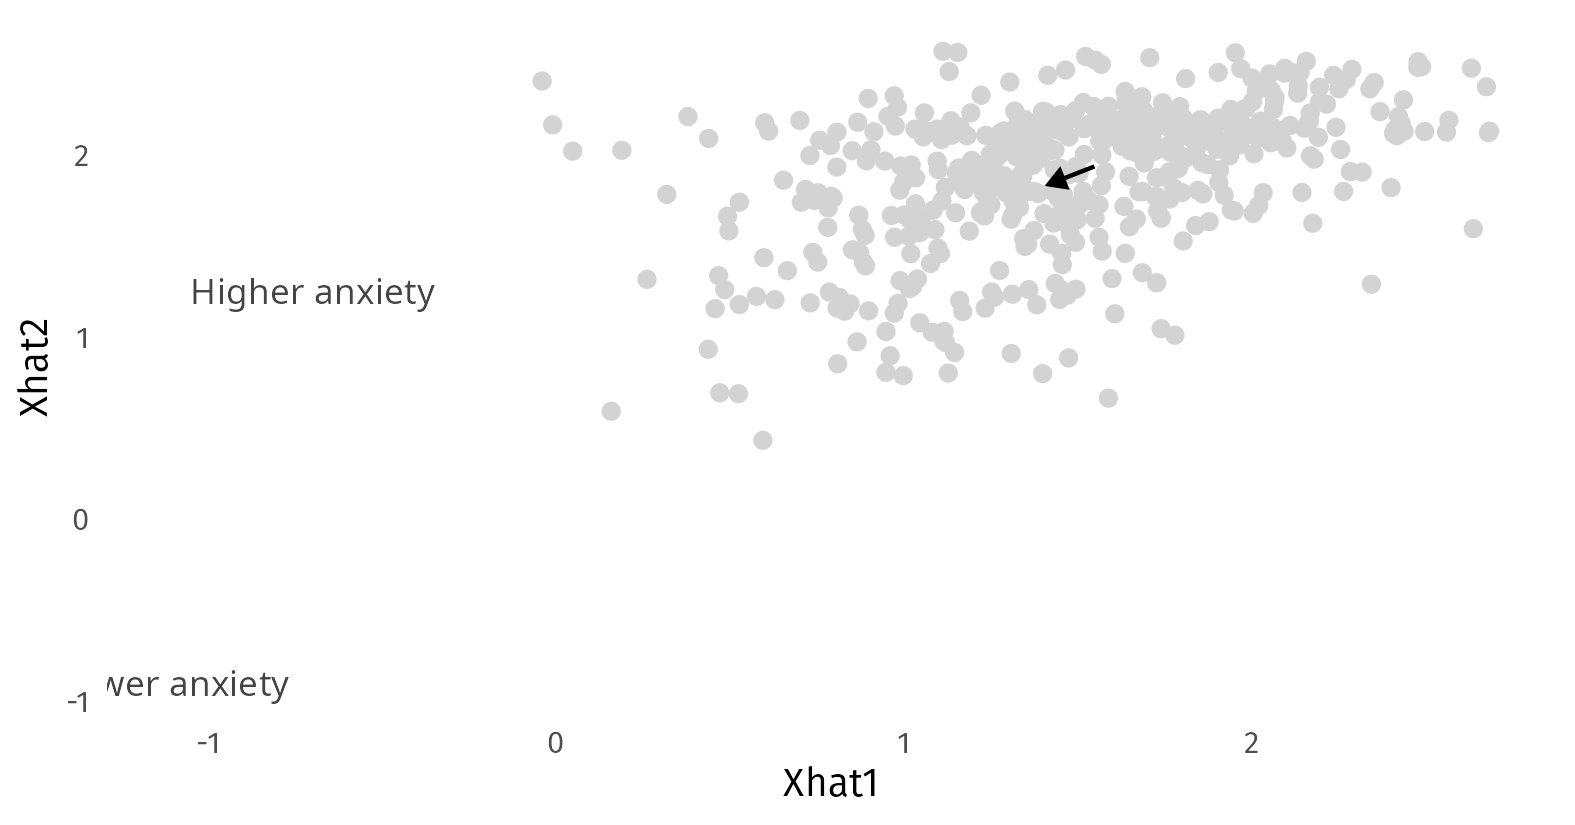
\includegraphics{figures/latent-intervention.png}
    \end{figure}
\end{frame}


\begin{frame}{We estimate that most of the effect is along the direct pathway}

    \begin{columns}
        \column{0.35\textwidth}
        \begin{align*}
            \atehat & = -2.7 \pm 1.3 \\
            \ndehat & = -1.8 \pm 1.1 \\
            \niehat & = -1 \pm 0.7
        \end{align*}

        \column{0.65\textwidth}
        \centering
        \begin{figure}[ht]
            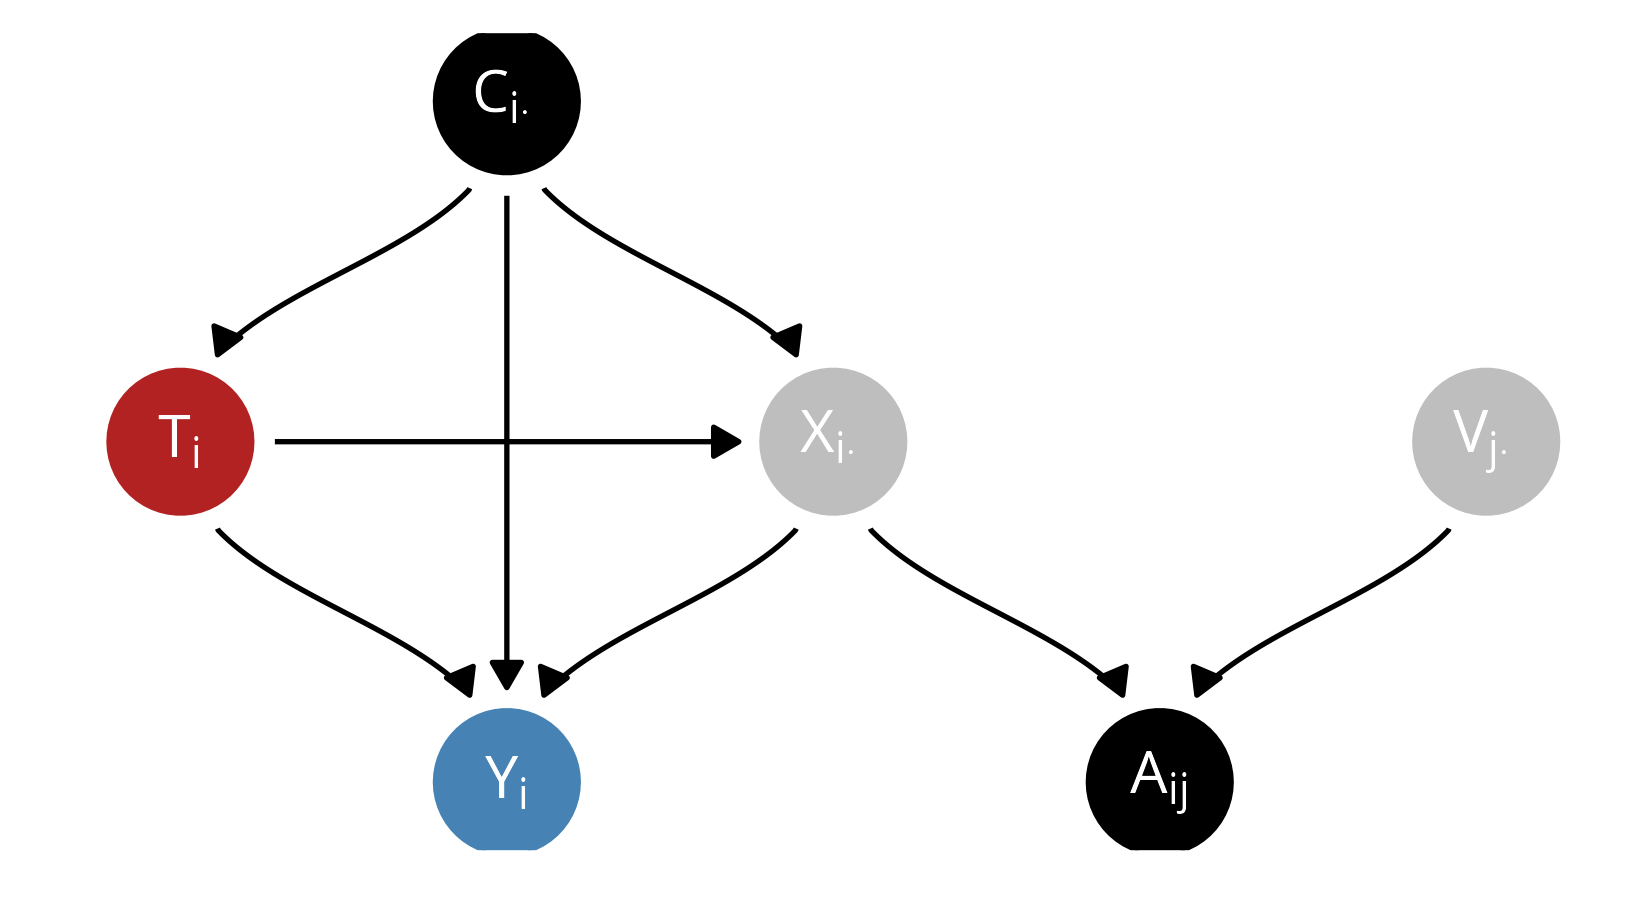
\includegraphics[width=\textwidth]{figures/dags/bipartite-mediation.png}
        \end{figure}
    \end{columns}
\end{frame}

\begin{frame}{Takeaways}

    \begin{itemize}
        \item We developed a method to decompose causal effects into effects operating along direct and indirect pathways in a low-rank latent space
        \item "Latent causal effects" sounds scary, but can often just look at your data to interpret them
    \end{itemize}

    \begin{columns}
        \column{0.3 \textwidth}
        \begin{align*}
            \ate    & = \nde + \nie  \\
            \atehat & = -2.7 \pm 1.3 \\
            \ndehat & = -1.8 \pm 1.1 \\
            \niehat & = -1 \pm 0.7
        \end{align*}
        \column{0.7 \textwidth}
        \centering
        \begin{figure}[ht]
            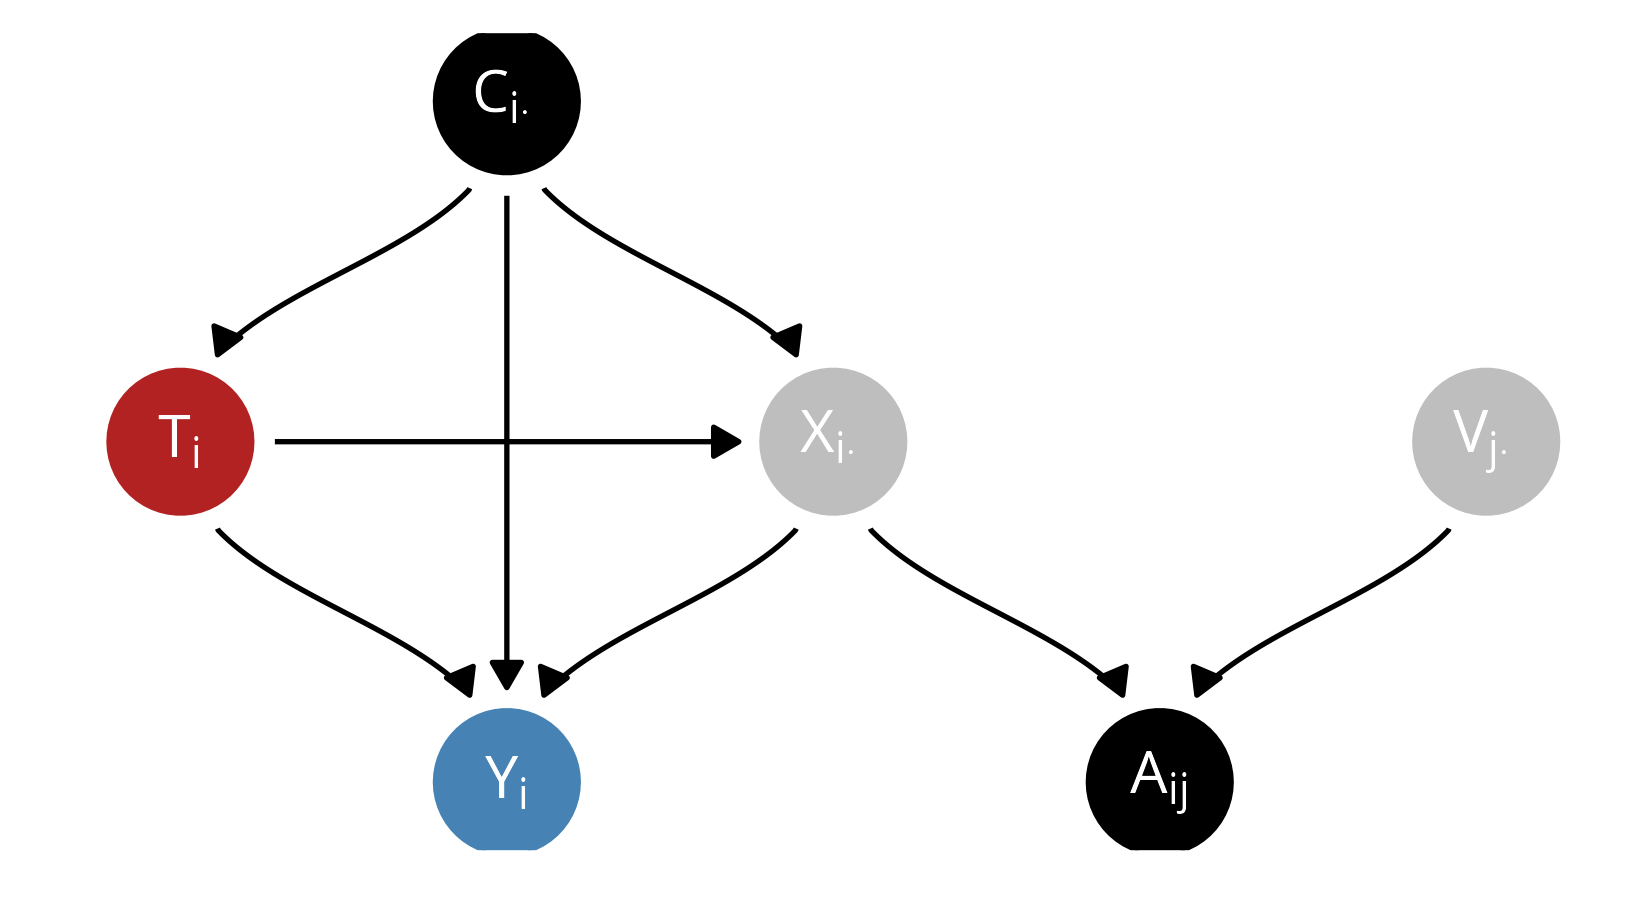
\includegraphics[width=\textwidth]{figures/dags/bipartite-mediation.png}
        \end{figure}
    \end{columns}
\end{frame}

% Visualize shift caused by intervention in latent space // how anxiety varies in that latent space



% \begin{frame}{We propose a model where social groups in networks mediate causal effects}

%     \begin{columns}

%         \column{0.35 \textwidth}

%         \footnotesize

%         \begin{table}[]
%             \begin{tabular}{lcl}
%                 Adjacency matrix      & $A$            & $\in \R^{n \times n}$ \\
%                 Edge $i \sim j$       & $A_{ij}$       & $\in \R$              \\
%                 Treatment             & $T_i$          & $\in \set{0, 1}$      \\
%                 Outcome               & $Y_i$          & $\in \R$              \\
%                 Confounders           & $\C_{i \cdot}$ & $\in \R^{1 \times p}$ \\
%                 Friend group (latent) & $\X_{i \cdot}$ & $\in \R^{1 \times d}$
%             \end{tabular}
%         \end{table}

%         \column{0.65 \textwidth}

%         \begin{figure}[ht]
%             \centering
%             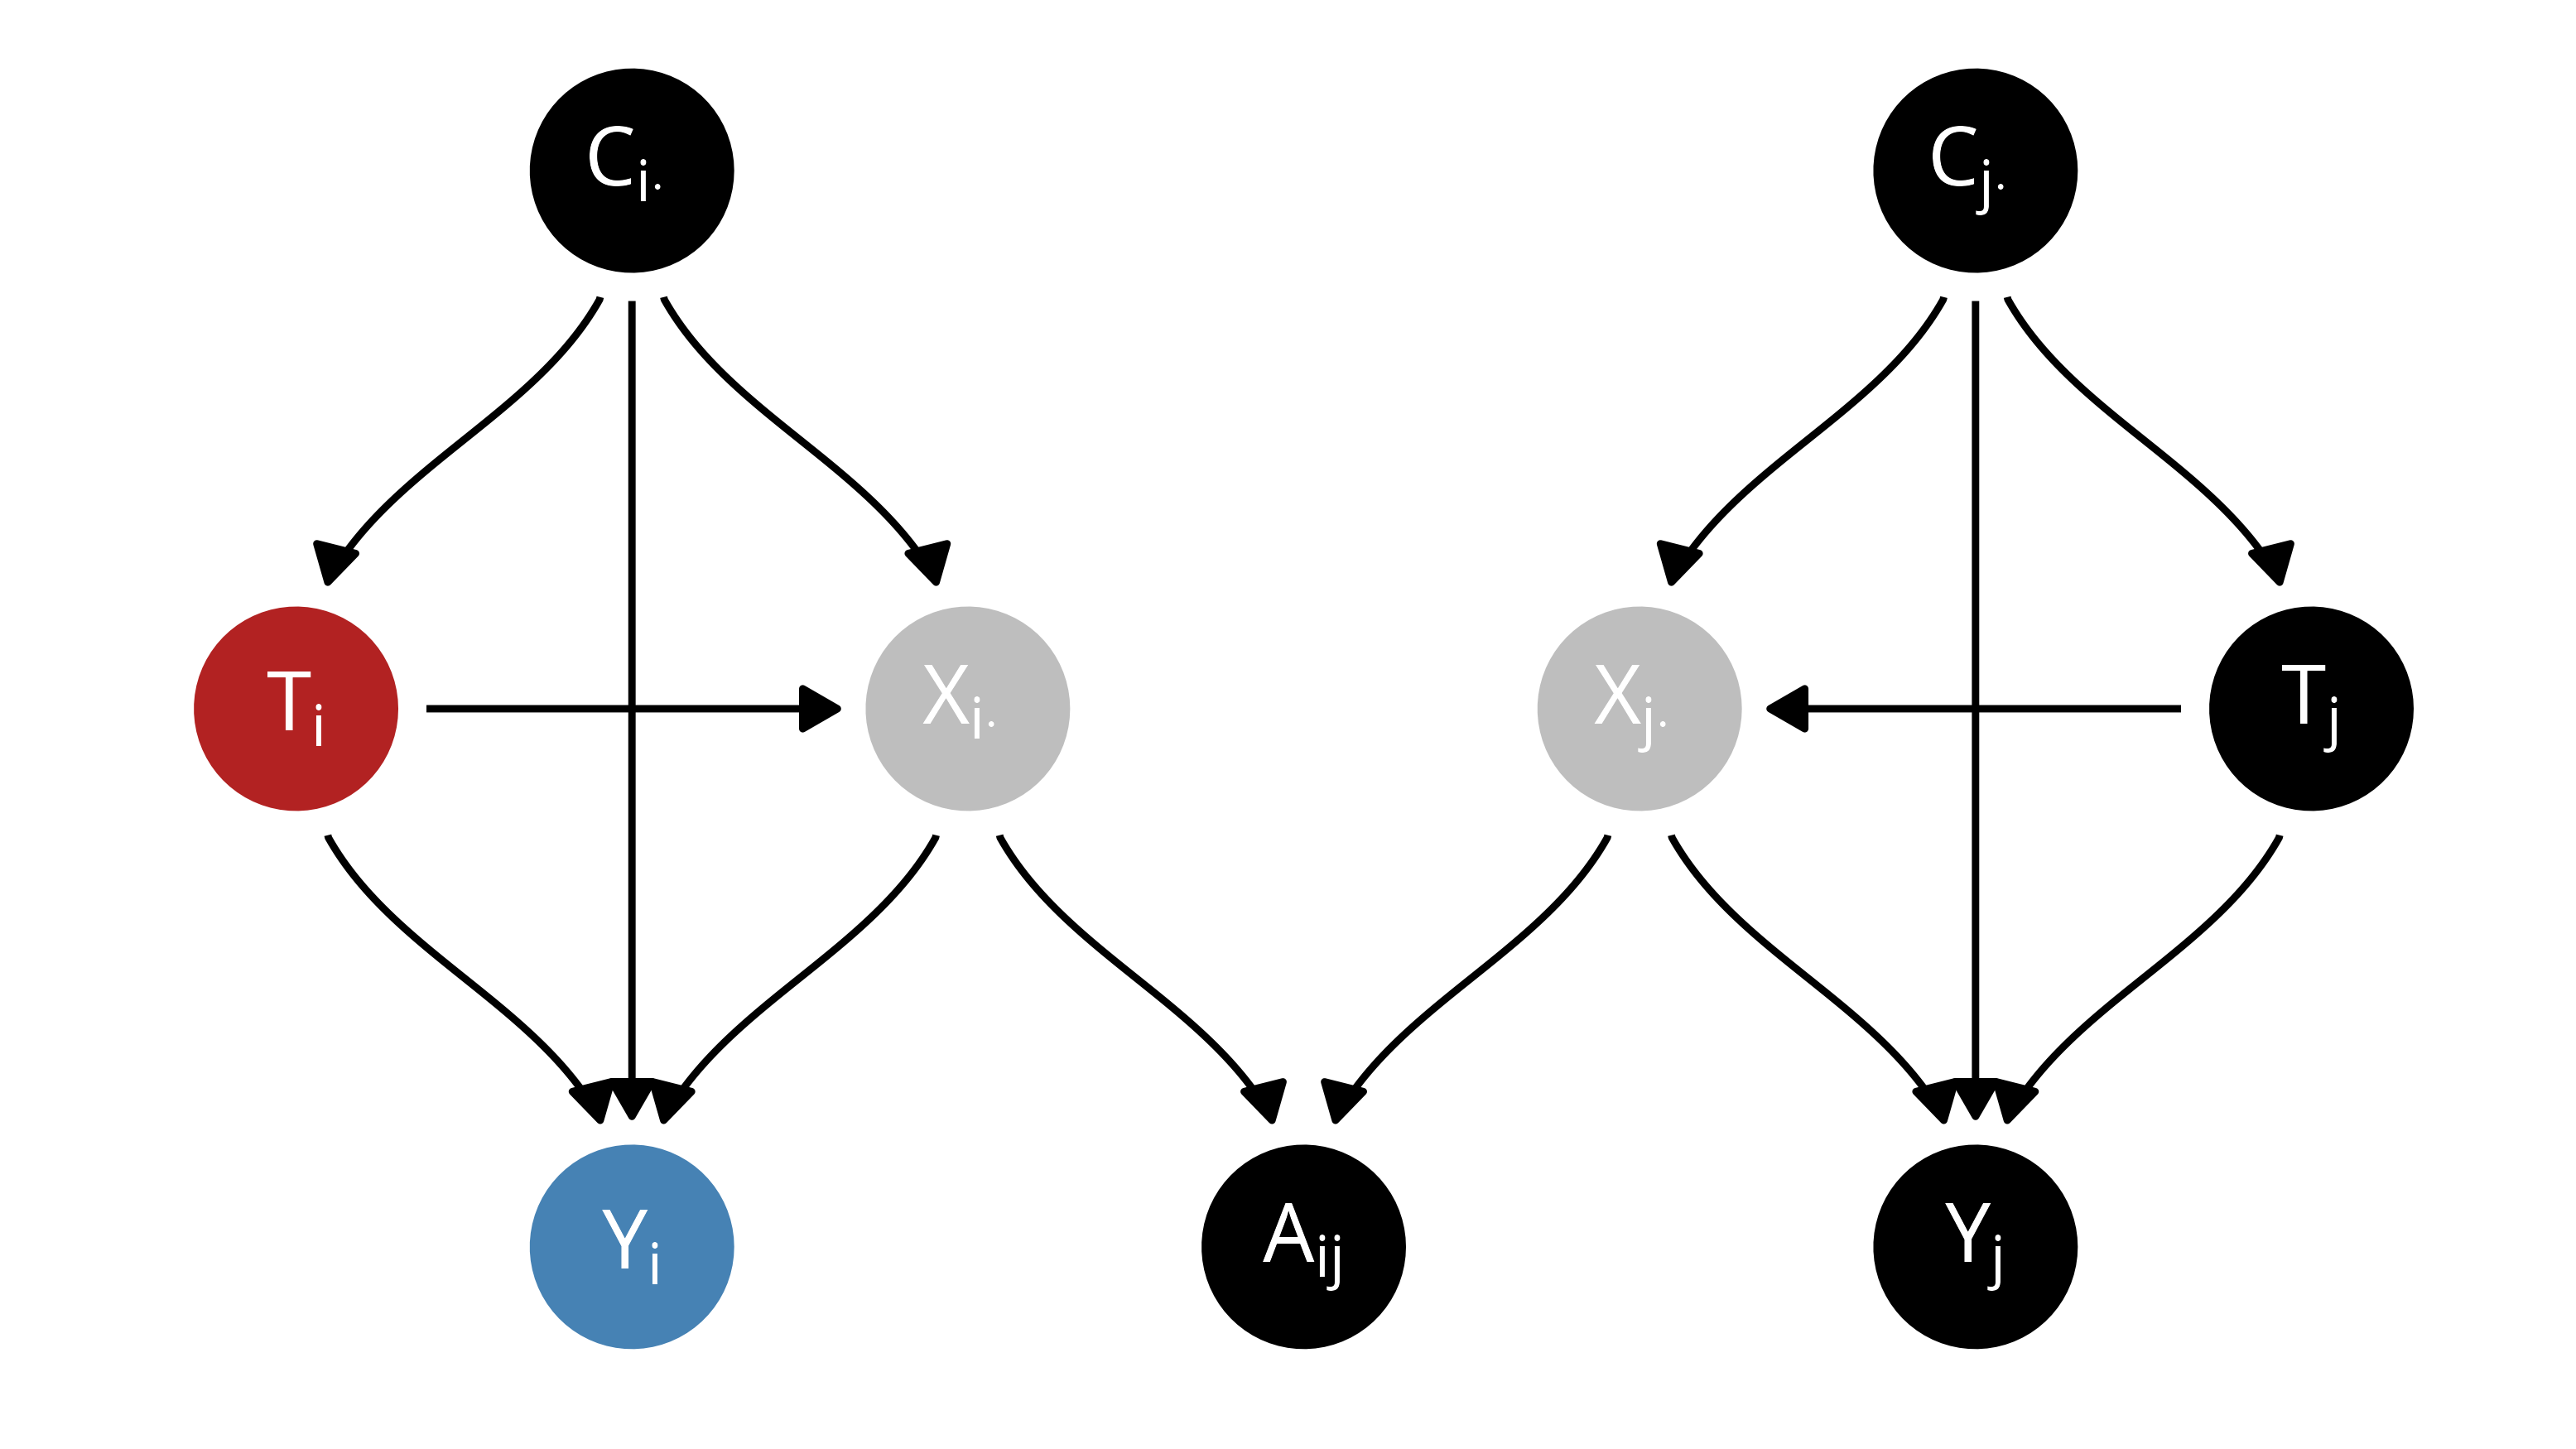
\includegraphics[width=\textwidth]{figures/dags/homophily-mediating.png}
%             \label{fig:mediating}
%         \end{figure}
%     \end{columns}

%     \centering
%     \scriptsize Structural causal model for network mediation in a network with two nodes $i$ and $j$


%     % \textbf{Motivating example:} friend groups mediate the effect of sex on smoking in an adolescent social network

%     % \begin{itemize}
%     %     \item Girls smoke than boys
%     %     \item Girls and boys in different friend groups
%     %     \item Smoking varies with friend group
%     % \end{itemize}


% \end{frame}

\begin{frame}{Thank you! Questions?}

    Read the manuscript at \url{https://arxiv.org/abs/2212.12041}

    R package \href{https://github.com/alexpghayes/latentnetmediate}{latentnetmediate}

    \textbf{Stay in touch}

    \begin{itemize}
        \item[] \faIcon{twitter} \href{https://twitter.com/alexpghayes}{@alexpghayes}
        \item[] \faIcon[regular]{envelope} \href{mailto:alex.hayes@wisc.edu}{alex.hayes@wisc.edu}
        \item[] \faIcon{wordpress} \url{https://www.alexpghayes.com} % \faIcon{sitemap} \faIcon{firefox-browser} 
        \item[] \faIcon{github} \url{https://github.com/alexpghayes}
    \end{itemize}

    \textbf{I'm looking for a post-doc starting Fall 2024, say hi if this work interests you!}
\end{frame}

\appendix

% \begin{frame}{Disambiguation: contagion ($Y_j \to Y_i$) is not allowed}

%     \centering

%     \begin{figure}
%         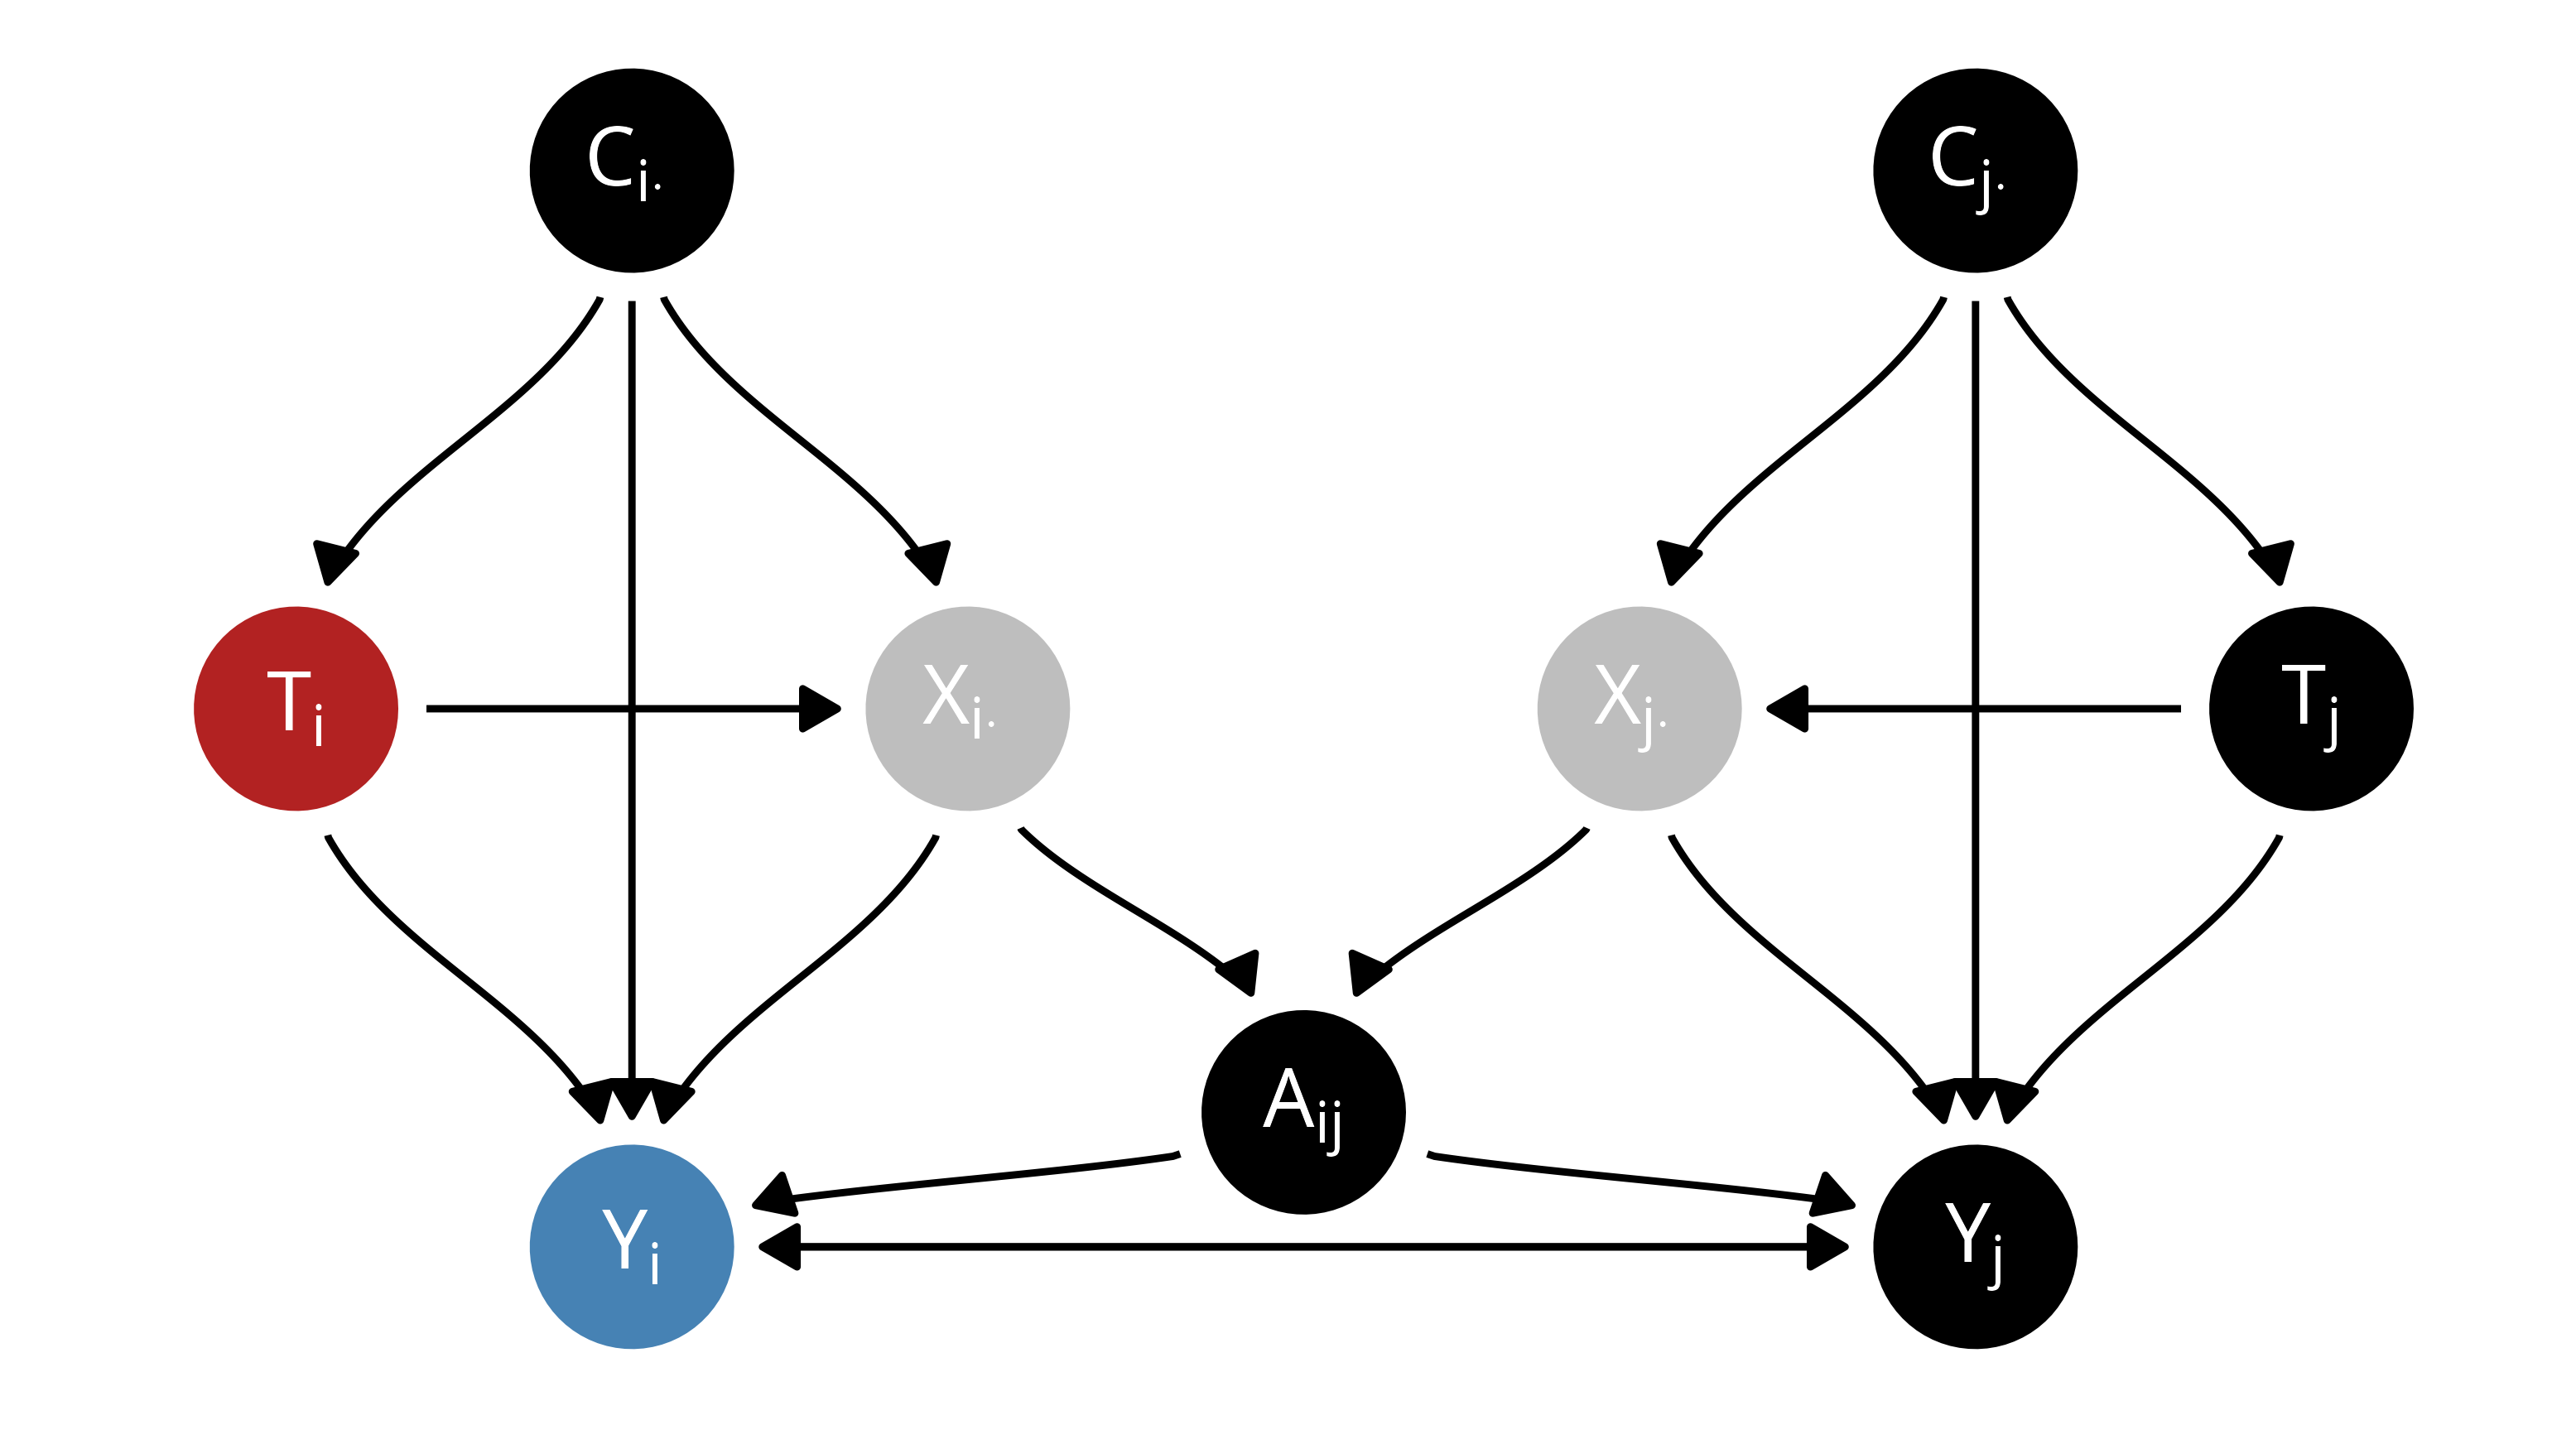
\includegraphics[scale=0.7]{figures/dags/homophily-mediating-contagion-peer.png}
%         \label{fig:contagion}
%     \end{figure}

% \end{frame}

% \begin{frame}{Disambiguation: interference ($T_j \to Y_i$) is not allowed}

%     \centering

%     \begin{figure}
%         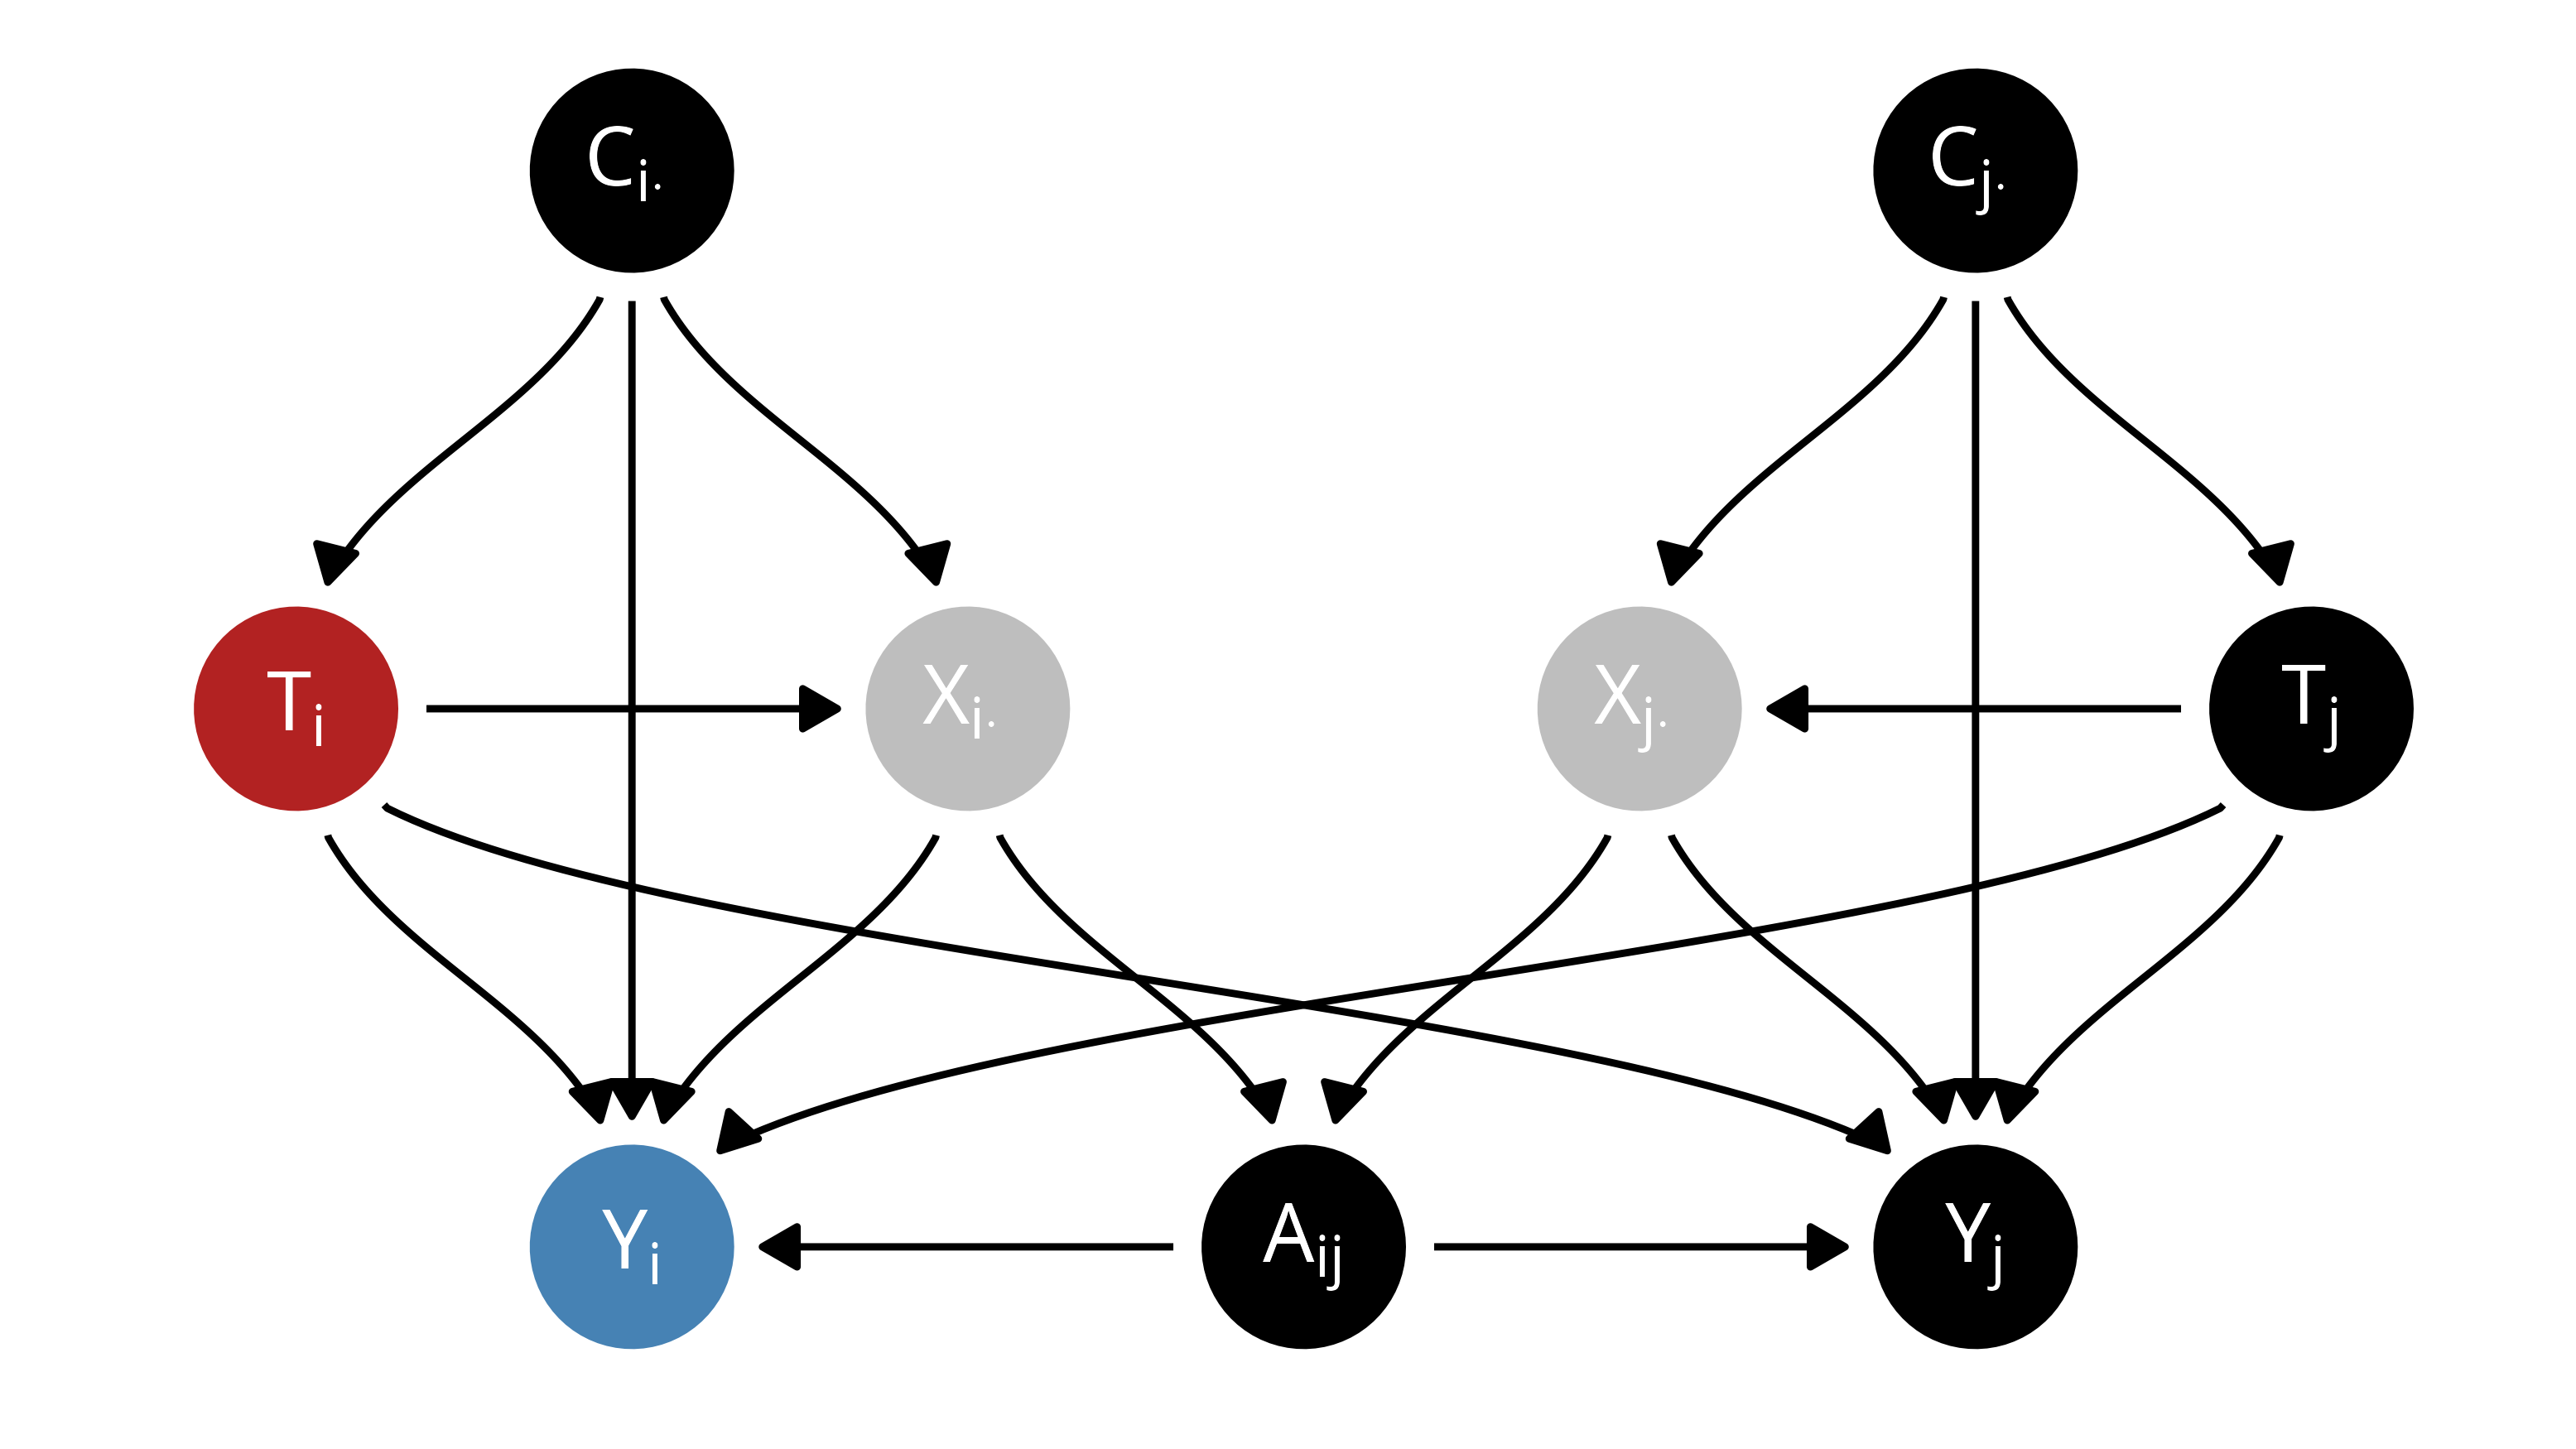
\includegraphics[scale=0.7]{figures/dags/homophily-mediating-interference-peer.png}
%         \label{fig:interference}
%     \end{figure}

% \end{frame}

% \begin{frame}{More on interference and contagion}

%     Interference and contagion effects are allowed \emph{so long as they happen in the latent space}. Suppose
%     \begin{align*}
%         \E[\W_{i \cdot}, \X_{i \cdot}]{Y_i}
%         = \W_{i \cdot} \betaw + \X_{i \cdot} \beta'_\text{x} + \delta_\text{y} \sum_{j} \X_{i \cdot}^T \X_{j \cdot} Y_j
%     \end{align*}
%     This latent space contagion model is a special parametric case of the regression outcome model (take $\betax = \beta'_\text{x} + \X^T Y \delta_\text{y}$).

% \end{frame}

\begin{frame}{Semi-parametric network model}

    \begin{definition}
        Let $A \in \R^{n \times n}$ be a random symmetric matrix, such as the adjacency matrix of an undirected graph. Let $\Apop = \E[\X]{A} = \X \X^T$ be the expectation of $A$ conditional on $\X \in \R^{n \times d}$, which has independent and identically distributed rows $\X_{1 \cdot}, \dots, \X_{n \cdot}$. That is, $\Apop$ has $\rank \paren*{\Apop} = d$ and is positive semi-definite with eigenvalues $\lambda_1 \ge \lambda_2 \ge \cdots \ge \lambda_d > 0 = \lambda_{d+1} = \cdots = \lambda_n$. Conditional on $\X$, the upper-triangular elements of $A - \Apop$ are independent $(\nu_n, b_n)$-sub-gamma random variables.
    \end{definition}

    \begin{remark}
        $\Apop = \X \X^T = (\X Q) (\X Q)^T$ for any $d \times d$ orthogonal matrix $Q$, the latent positions $\X$ are only identifiable up to an orthogonal transformation.
    \end{remark}

\end{frame}

\begin{frame}{Choosing $\widehat{d}$: overestimating the embedding dimension is fine}

    \centering

    \begin{figure}
        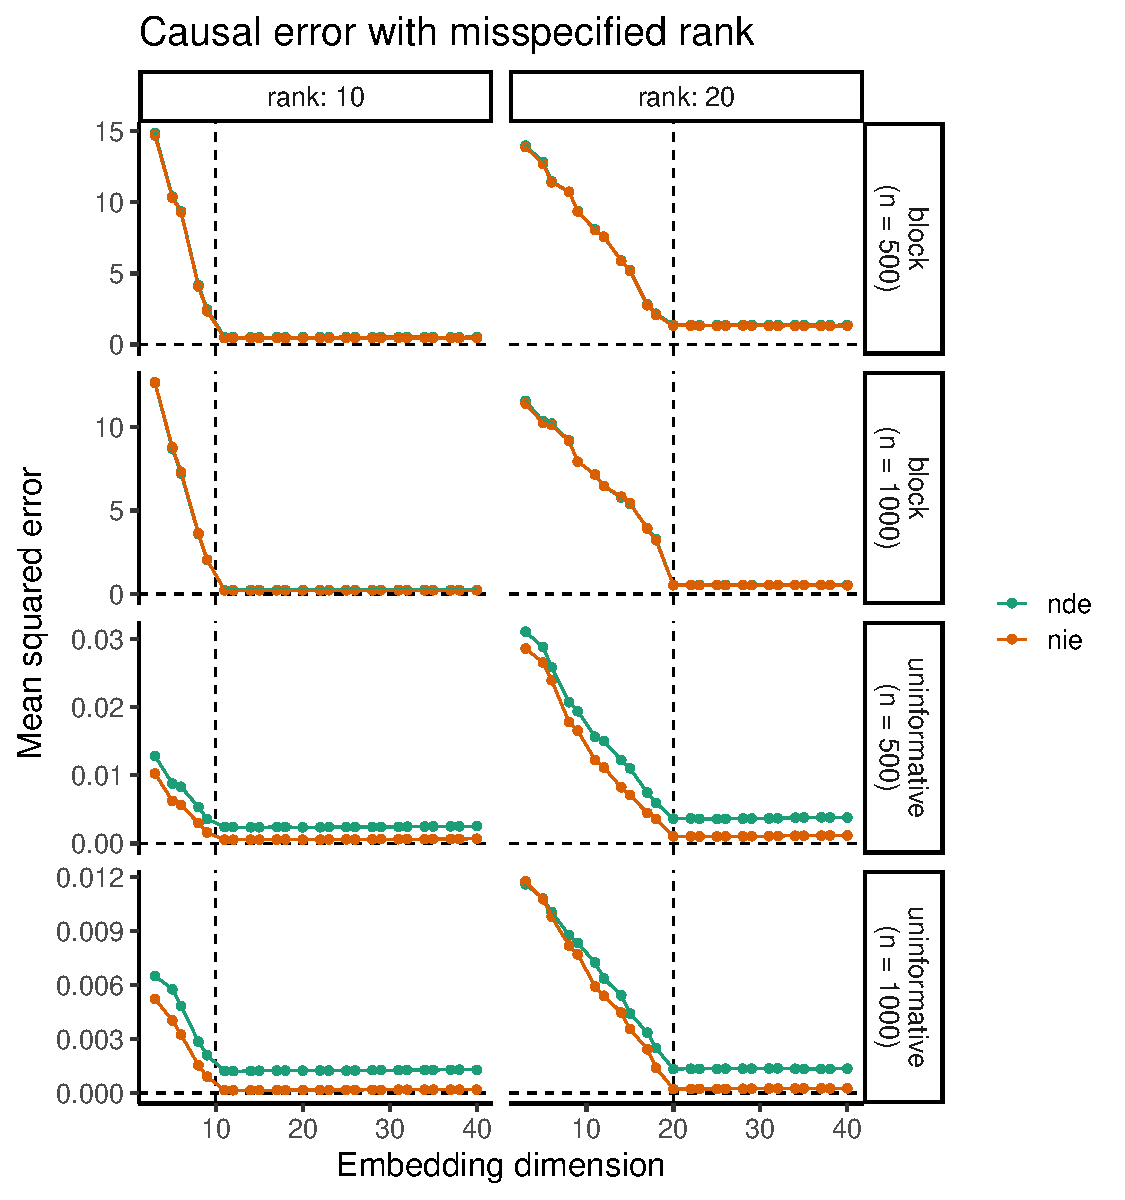
\includegraphics[width=0.5\textwidth]{figures/misspecification/loss_average.pdf}
    \end{figure}

\end{frame}


% % \begin{frame}{Interventions on a network}

% %     \begin{figure}
% %         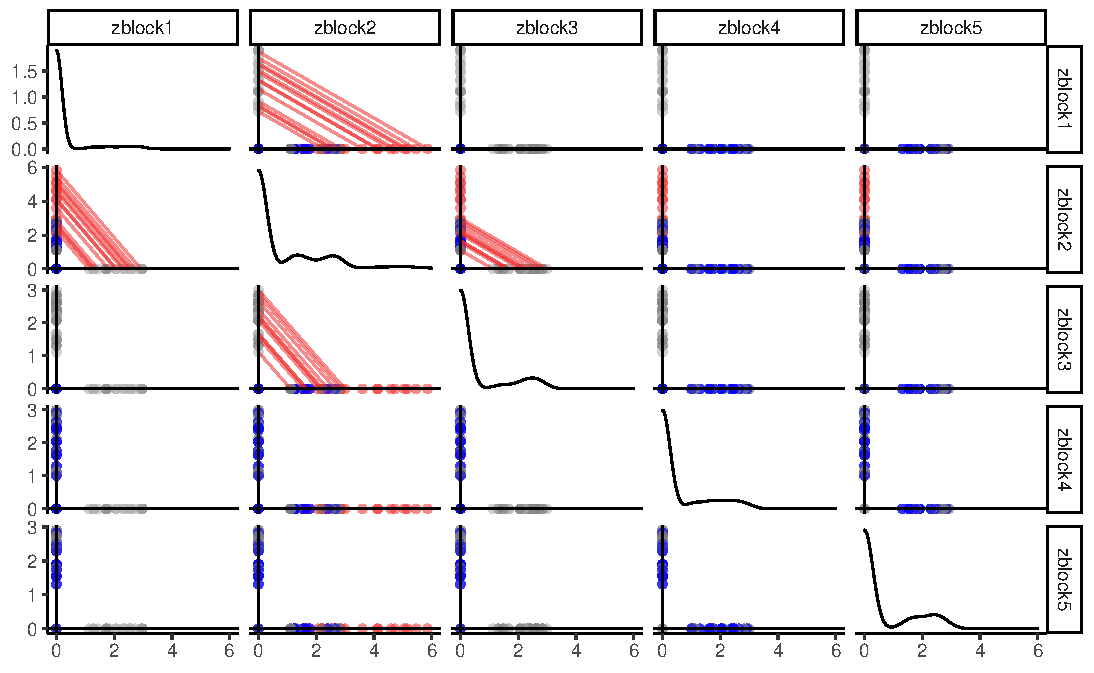
\includegraphics[width=\textwidth]{figures/intervention.pdf}
% %         \caption{Canonical intervention when $\C$ is highly informative.}
% %         \label{fig:intervention}
% %     \end{figure}
% % \end{frame}

% % \begin{frame}{Interventions on a network}

% %     \begin{align*}
% %         \underbrace{\E[T_i, \C_{i \cdot}]{\Z_{i \cdot}}}_{\R^{1 \times d}}
% %          & = \underbrace{\thetazero}_{\R^{1 \times d}}
% %         + \underbrace{T_i}_{\{0, 1\}} \underbrace{\thetat}_{\R^{1 \times d}}
% %         + \underbrace{\C_{i \cdot}}_{\R^{1 \times p}} \underbrace{\Thetac}_{\R^{p \times d}}
% %         + \underbrace{T_i}_{\{0, 1\}} \underbrace{\C_{i \cdot}}_{\R^{1 \times p}} \underbrace{\Thetatc}_{\R^{p \times d}}.
% %     \end{align*}

% %     In Figure \ref{fig:intervention}, $\C$ are latent parameters for a DC-SBM and $\thetazero = \vec 0, \thetat = \vec 0, \Thetac = I_k$ and

% %     \begin{align*}
% %         \Thetatc =
% %         \begin{bmatrix}
% %             -1 & 2 & 0  & 0 & 0 \\
% %             0  & 0 & 0  & 0 & 0 \\
% %             0  & 1 & -1 & 0 & 0 \\
% %             0  & 0 & 0  & 0 & 0 \\
% %             0  & 0 & 0  & 0 & 0 \\
% %         \end{bmatrix}
% %     \end{align*}
% % \end{frame}

% \begin{frame}{Interventions allowed}

%     Provided that controls $\C_{i \cdot}$ are sufficiently informative about group membership $\X_{i \cdot}$, treatment $T_i$ is allowed to cause:

%     \begin{itemize}
%         \item Changes in popularity within a group
%         \item Movement to a new friend group
%         \item Becoming a member of a new friend group while remaining in current friend group
%         \item Friendships becoming more or less likely between distinct friend groups
%         \item Combinations of the above
%     \end{itemize}

%     See Appendix of manuscript for details.

% \end{frame}

\begin{frame}{mindful action subscale}

    \begin{enumerate}
        \item When I do things, my mind wanders off and I'm easily distracted.
        \item I don't pay attention to what I'm doing because I'm daydreaming, worrying, or otherwise distracted.
        \item I am easily distracted.
        \item I find it difficult to stay focused on what's happening in the present.
        \item It seems I am 'running on automatic' without much awareness of what I'm doing.
        \item I rush through activities without being really attentive to them.
        \item I do jobs or tasks automatically without being aware of what I'm doing.
        \item I find myself doing things without paying attention.
    \end{enumerate}

    \resizebox{\linewidth}{!}{
        \begin{tabular}{ccccc}
            Never or very rarely true  & Rarely true                & Sometimes true             & Often true                 & Very often or always true  \\
            1 \faIcon[regular]{circle} & 2 \faIcon[regular]{circle} & 3 \faIcon[regular]{circle} & 4 \faIcon[regular]{circle} & 5 \faIcon[regular]{circle}
        \end{tabular}
    }
\end{frame}



\begin{frame}{Drexel Defusion Scale}
    \begin{enumerate}
        \item Feelings of anger. You become angry when someone takes your place in a long line. To what extent would you normally be able to defuse from feelings of anger?
        \item Cravings for food. You see your favorite food and have the urge to eat it. To what extent would you normally be able to defuse from cravings for food?
        \item Physical pain. Imagine that you bang your knee on a table leg. To what extent would you normally be able to defuse from physical pain?
        \item Anxious thoughts. Things have not been going well at school or your job, and work just keeps piling up. To what extent would you normally be able to defuse from anxious thoughts like "I'll never get this done."?
        \item Thoughts of self. Imagine you are having a thought such as "no one likes me." To what extent would you normally be able to defuse from negative thoughts about yourself?
        \item Thoughts of hopelessness. You are feeling sad and stuck in a difficult situation that has no obvious end in sight. You experience thoughts such as "Things will never get any better." To what extent would you normally be able to defuse from thoughts of hopelessness?
        \item Thoughts about motivation or ability. Imagine you are having a thought such as "I can't do this" or "I just can't get started." To what extent would you normally be able to defuse from thoughts about motivation or ability?
        \item Thoughts about your future. Imagine you are having thoughts like, "I'll never make it" or "I have no future." To what extent would you normally be able to defuse from thoughts about your future?
        \item Sensations of fear. You are about to give a presentation to a large group. As you sit waiting for your turn, you start to notice your heart racing, butterflies in your stomach, and your hands trembling. To what extent would you normally be able to defuse from sensations of fear?
        \item Feelings of sadness. Imagine that you lose out on something you really wanted. You have feelings of sadness. To what extent would you normally be able to defuse from feelings of sadness?
    \end{enumerate}

    \resizebox{\linewidth}{!}{
        \begin{tabular}{cccccc}
            Not at all                 & A little                   & Somewhat                   & Moderately                 & Quite a lot                & Very much                  \\
            0 \faIcon[regular]{circle} & 1 \faIcon[regular]{circle} & 2 \faIcon[regular]{circle} & 3 \faIcon[regular]{circle} & 4 \faIcon[regular]{circle} & 5 \faIcon[regular]{circle}
        \end{tabular}
    }

\end{frame}

\begin{frame}{Network model}


    \begin{definition}
        Let $A \in \R^{n \times n}$ be a random symmetric matrix, such as the adjacency matrix of an undirected graph. Let $\Apop = \E[\X]{A} = \X \X^T$ be the expectation of $A$ conditional on $\X \in \R^{n \times d}$, which has independent and identically distributed rows $\X_{1 \cdot}, \dots, \X_{n \cdot}$. That is, $\Apop$ has $\rank \paren*{\Apop} = d$ and is positive semi-definite with eigenvalues $\lambda_1 \ge \lambda_2 \ge \cdots \ge \lambda_d > 0 = \lambda_{d+1} = \cdots = \lambda_n$. Conditional on $\X$, the upper-triangular elements of $A - \Apop$ are independent $(\nu_n, b_n)$-sub-gamma random variables.
    \end{definition}

    \begin{remark}
        $\Apop = \X \X^T = (\X Q) (\X Q)^T$ for any $d \times d$ orthogonal matrix $Q$, the latent positions $\X$ are only identifiable up to an orthogonal transformation.
    \end{remark}

\end{frame}

% \bibliographystyle{chicago}
% \bibliography{2024-06-17-netsci}

\end{document}